% ============================================================
% DRL Portfolio — Rapport pédagogique (cheminement complet)
% Compiler :  tectonic rapport_drl_portfolio.tex   (ou Overleaf)
% Les figures sont générées par :  python reports/build_assets.py
% ============================================================
\documentclass[11pt,a4paper]{article}

\usepackage[french]{babel}
\usepackage[margin=2.4cm]{geometry}
\usepackage{graphicx}
\usepackage{booktabs}
\usepackage{amsmath}
\usepackage{amssymb}
\usepackage{xcolor}
\usepackage{float}
\usepackage{caption}
\usepackage{enumitem}
\usepackage[colorlinks=true, linkcolor=blue!50!black, urlcolor=blue!50!black]{hyperref}

\graphicspath{{figures/}}
\captionsetup{font=small, labelfont=bf}

\definecolor{okgreen}{HTML}{1E8449}
\definecolor{kored}{HTML}{C0392B}

\newcommand{\ok}[1]{\textcolor{okgreen}{#1}}
\newcommand{\ko}[1]{\textcolor{kored}{#1}}
\newcommand{\code}[1]{\texttt{#1}}

\title{\textbf{DRL Portfolio} \\[4pt]
\large Un agent de trading par apprentissage par renforcement profond : \\
mon cheminement, mes erreurs, mes corrections, mes résultats \\[6pt]
\normalsize Rapport pédagogique --- version du 3 juillet 2026}
\author{Martin Chassaing \\ \small IMT Atlantique \& Université Paris Dauphine}
\date{}

\begin{document}
\maketitle

\begin{abstract}
Ce rapport retrace la construction d'un agent de trading par \emph{Deep Reinforcement
Learning} (PPO) sur données journalières réelles, en suivant le cheminement réel du
projet : ce que j'ai essayé, ce qui n'a pas fonctionné, pourquoi, et ce que chaque
constat m'a poussé à faire ensuite. Sur un test set jamais vu à l'entraînement (février
2021 $\to$ décembre 2022), l'agent multi-actifs réalise $+23{,}8\,\%$ contre
$-3{,}7\,\%$ pour le Buy \& Hold (alpha $+27{,}5\,\%$), avec un alpha positif sur les
cinq actifs testés. Mais la validation \emph{walk-forward} (25 cellules année$\times$actif
out-of-sample) que j'ai menée ensuite relativise ce chiffre : l'agent a un profil
\emph{défensif régime-dépendant} --- rendement absolu positif 4 années sur 5 et alpha
fortement positif dans les marchés baissiers, mais retard net sur le B\&H dans les
fortes hausses. Chaque étape est reliée aux notions d'économétrie (stationnarité,
GARCH, biais de look-ahead, validation out-of-sample) et de gestion de portefeuille
(alpha de Jensen, Sharpe, Sortino, CVaR, drawdown). Enfin, deux stress-tests que je me
suis imposés --- sensibilité aux frais et ablation du kill-switch --- montrent que
l'essentiel de l'alpha 2022 provient de la règle de stop : un alpha de \emph{gestion du
risque} plus que de signal, distinction que j'assume et documente. Projet strictement
éducatif.
\end{abstract}

\tableofcontents
\vspace{1em}

% ============================================================
\section{Objectif et démarche}
% ============================================================

Je suis parti d'une question simple : \emph{un agent d'apprentissage par renforcement
peut-il apprendre à battre une stratégie passive (Buy \& Hold) sur données réelles, une
fois les frais de transaction pris en compte ?}

\paragraph{Pourquoi cette question n'est pas naïve : l'efficience des marchés.}
Mon agent n'observe \emph{que} des transformations de prix passés (rendements,
volatilité, momentum\ldots). Or l'hypothèse d'efficience des marchés dans sa
\textbf{forme faible} (Fama, 1970) affirme précisément que les prix intègrent déjà
toute l'information contenue dans leur propre historique : aucune stratégie fondée sur
les prix passés ne devrait battre durablement le marché \emph{après coûts}. Ce projet
est donc, littéralement, \textbf{un test empirique de l'efficience faible} sur mon
échantillon. Et son résultat final est cohérent avec la littérature : pas de machine à
cash, mais un edge modeste, défensif, dépendant du régime et majoritairement porté par
une règle de risque --- le même genre de « violation limite » que les anomalies
documentées (momentum de Jegadeesh-Titman en tête). Savoir formuler le projet ainsi
change tout : je ne prétends pas avoir réfuté Fama, je mesure \emph{où} et \emph{de
combien} l'hypothèse craque sur cinq actifs et treize ans.

\paragraph{Pourquoi du RL, et pas de la prédiction supervisée ?} L'alternative évidente
serait un modèle supervisé qui prédit le rendement de demain, suivi d'une règle de
trading. Deux raisons m'ont fait préférer le RL : (1) la décision de trading est
\emph{séquentielle et porteuse d'état} --- ma position d'aujourd'hui conditionne mes
frais de demain (fermer puis rouvrir coûte deux fois) : optimiser la qualité de
prédiction n'optimise pas la politique de trading, qui doit arbitrer signal contre
coûts de changement de position ; (2) mon objectif réel --- l'alpha net de frais sous
contrainte de drawdown --- s'écrit naturellement comme une fonction de récompense, pas
comme une erreur quadratique de prévision. Le RL optimise directement ce que je veux
maximiser ; le supervisé optimise un substitut.

À la fin du parcours, ma réponse tient en trois temps, et c'est ce cheminement que ce
rapport documente :
\begin{enumerate}[itemsep=2pt]
  \item mes premiers résultats semblaient bons mais étaient \textbf{invalides} --- pas
        parce que le modèle était mauvais, mais parce que mon protocole d'évaluation
        était faux (observations non normalisées, frais incohérents, validation
        corrompue) ;
  \item une fois le protocole corrigé et le modèle réentraîné, l'agent \textbf{bat
        nettement le B\&H} sur mon split de test, et généralise sur cinq actifs ;
  \item la validation walk-forward m'a ensuite appris que ce résultat était
        \textbf{partiellement un artefact de la période de test} : mon agent est
        défensif, brillant en marché baissier, à la traîne dans les fortes hausses.
\end{enumerate}

La leçon transversale : en finance quantitative, \emph{la qualité d'une conclusion vaut
celle du protocole qui la produit}. J'ai passé plus de temps à fiabiliser l'évaluation
qu'à optimiser le modèle --- et c'est l'évaluation qui a tout changé.

\paragraph{Ma méthode, en cinq règles.} Tout le rapport applique la même discipline ;
autant l'énoncer une fois pour toutes :
\begin{enumerate}[itemsep=2pt]
  \item \textbf{Fiabiliser avant d'optimiser} : un simulateur ou un protocole faux rend
        toute optimisation illisible --- les tests et les corrections passent avant les
        hyperparamètres.
  \item \textbf{Une prédiction écrite avant chaque expérience} : elle force à réfléchir
        avant de calculer, et une prédiction fausse enseigne plus qu'une juste (les
        miennes sont documentées, y compris les fausses).
  \item \textbf{Un levier à la fois} : quand plusieurs choses changent ensemble, une
        ablation contrôlée isole l'effet causal (tableaux~\ref{tab:ablationbug}
        et~\ref{tab:ablation}).
  \item \textbf{Aucune conclusion sans barre d'erreur} : un chiffre unique est un
        tirage ; la bande inter-seeds (section~\ref{sec:seeds}) est le juge de paix.
  \item \textbf{Chercher à se falsifier} : walk-forward, stress-tests, ablations ---
        si le résultat survit à mes propres attaques, alors seulement il mérite d'être
        présenté.
\end{enumerate}

% ============================================================
\section{Architecture du projet}
% ============================================================

\begin{table}[H]
\centering\small
\begin{tabular}{@{}llp{8.2cm}@{}}
\toprule
\textbf{Fichier} & \textbf{Rôle} & \textbf{Contenu} \\
\midrule
\code{data\_loader.py} & Données & Téléchargement yfinance, feature engineering,
normalisation \emph{fittée sur le train uniquement}, split temporel 70/15/15,
pipeline multi-actifs avec segments. \\
\code{environment.py} & Simulation & Environnement Gymnasium : 4 actions
(Hold/Long/Flat/Short), comptabilité exacte des frais, kill-switch drawdown,
épisodes confinés par actif. \\
\code{train.py} & Entraînement & PPO (Stable-Baselines3), 4 environnements parallèles,
normalisation des observations (\code{VecNormalize}), sélection du meilleur modèle
sur la validation. \\
\code{evaluate.py} & Évaluation & Protocole déterministe sur split complet, robustesse
sur sous-fenêtres, Sharpe/Sortino/Calmar/CVaR, diagnostic d'overfitting,
généralisation cross-actifs. \\
\code{walk\_forward.py} & Validation & Réentraînements glissants (fenêtre croissante
ancrée), une année de test 100\,\% out-of-sample par fold, grille année$\times$actif. \\
\code{dashboard.py} & Visualisation & Application Streamlit interactive. \\
\code{tests/} & Qualité & 74 tests pytest : pipeline de données, mécanique de trading,
conformité Gymnasium, entraînements PPO courts réels, évaluation, walk-forward,
dashboard. \\
\code{reports/} & Présentation & Ce rapport, les figures, \code{build\_assets.py}
(figures + dashboard statique \code{docs/index.html}). \\
\bottomrule
\end{tabular}
\caption{Organisation du dépôt.}
\end{table}

\begin{figure}[H]
\centering
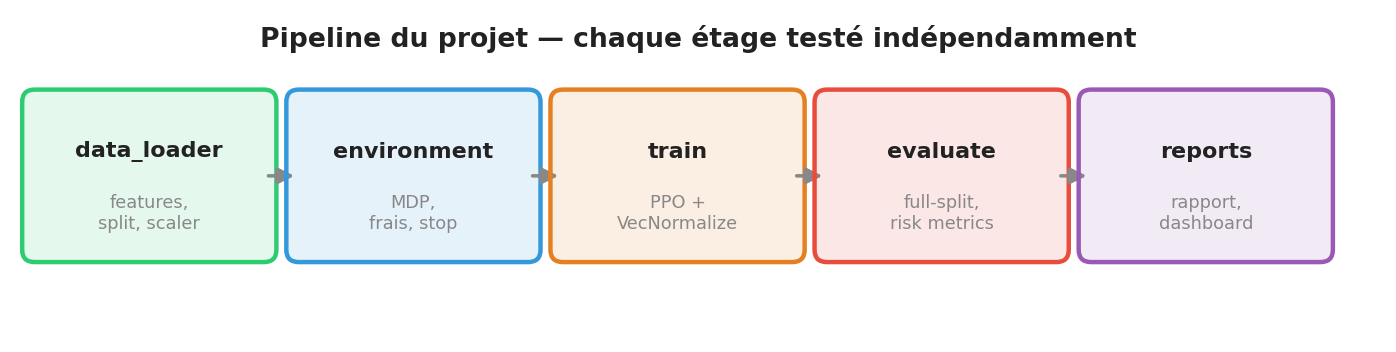
\includegraphics[width=\textwidth]{fig_pipeline.png}
\caption{Le flux du projet. Chaque étage est validé par des tests indépendants
(données synthétiques, sans réseau) avant d'être branché au suivant.}
\label{fig:pipeline}
\end{figure}

% ============================================================
\section{Base théorique : du RL au trading}
\label{sec:theorie}
% ============================================================

\subsection{Le trading comme processus de décision markovien}

L'apprentissage par renforcement modélise un \emph{processus de décision markovien}
(MDP) : à chaque jour de bourse $t$, l'agent observe un état $s_t$, choisit une action
$a_t$ selon sa politique $\pi(a_t \mid s_t)$, reçoit une récompense $r_t$, et
l'environnement transitionne vers $s_{t+1}$. L'objectif est de maximiser l'espérance de
la somme actualisée des récompenses $\mathbb{E}\big[\sum_t \gamma^t r_t\big]$, avec
$\gamma = 0{,}99$ : l'agent « voit » environ $1/(1-\gamma) = 100$ jours devant lui, un
horizon cohérent avec du trading journalier.

Deux termes que j'emploierai partout : un \textbf{épisode} est une traversée de la
simulation, du point de départ jusqu'à la fin des données ou au déclenchement du stop ;
une \textbf{seed} est la graine du générateur pseudo-aléatoire --- la fixer rend chaque
expérience exactement reproductible (indispensable pour comparer deux versions du code
à conditions identiques).

\begin{figure}[H]
\centering
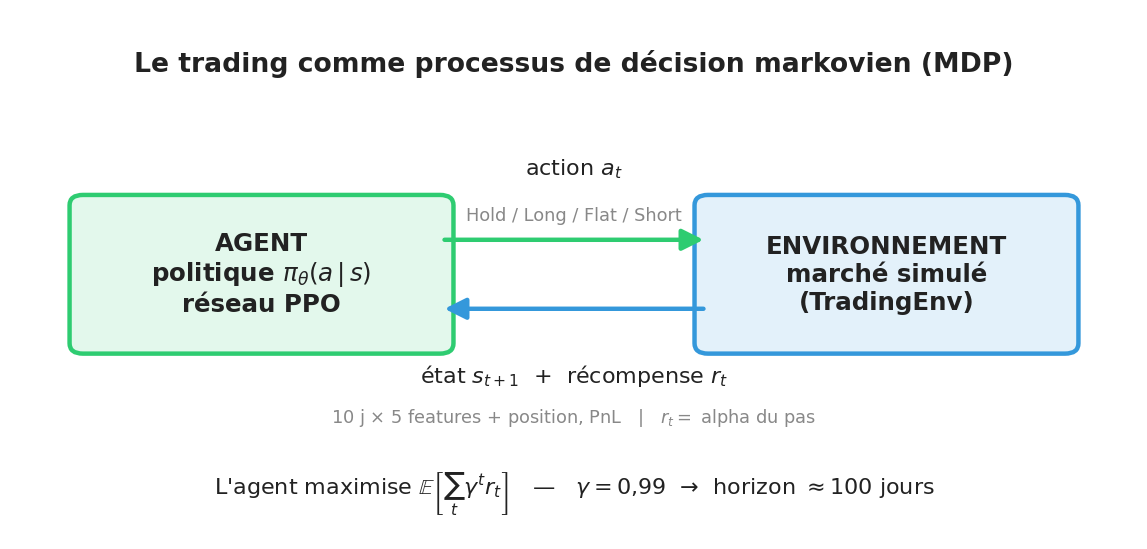
\includegraphics[width=0.9\textwidth]{fig_mdp_loop.png}
\caption{La boucle fondamentale du RL. À chaque jour de bourse, l'agent lit un état,
choisit une action, la passe à l'environnement, qui renvoie le nouvel état et une
récompense. Tout le reste du rapport n'est qu'un remplissage de plus en plus soigné de
ces quatre cases.}
\label{fig:mdp}
\end{figure}

\paragraph{Observation.} Une fenêtre glissante de 10 jours $\times$ 5 features de marché
(section~\ref{sec:features}), plus deux variables de portefeuille : la position courante
($-1$ short, $0$ cash, $+1$ long) et le PnL latent. Soit $10 \times 5 + 2 = 52$ entrées.
Remarque théorique honnête : les prix de marché ne sont évidemment pas markoviens dans
une fenêtre de 10 jours --- l'hypothèse MDP est une approximation, partiellement
compensée par des features qui résument le passé (volatilité, momentum).

\paragraph{Actions.} $\{$Hold, Long, Flat, Short$\}$. Le short est essentiel : sans lui,
le mieux qu'un agent puisse faire dans un marché baissier est de \emph{ne pas perdre}
(rester cash) ; avec lui, il peut \emph{gagner} pendant les baisses --- c'est exactement
ce qui se produit en 2022 (figure~\ref{fig:equity}).

\subsection{PPO en deux idées}

PPO (\emph{Proximal Policy Optimization}) est un algorithme de \emph{policy gradient} :
un réseau de neurones (ici volontairement petit, $2 \times 64$) produit directement la
distribution sur les actions, améliorée par montée de gradient sur l'avantage estimé
$A_t$ (« cette action a-t-elle rapporté plus que ce que la valeur de l'état laissait
espérer ? »). Sa spécificité est le \emph{clipping} :
\[
L(\theta) = \mathbb{E}_t\!\left[\min\!\big(\rho_t(\theta) A_t,\;
\operatorname{clip}(\rho_t(\theta),\, 1-\varepsilon,\, 1+\varepsilon)\, A_t\big)\right],
\qquad \rho_t(\theta) = \frac{\pi_\theta(a_t \mid s_t)}{\pi_{\theta_{\text{old}}}(a_t \mid s_t)},
\]
qui borne l'ampleur de chaque mise à jour de politique (ici $\varepsilon = 0{,}15$).
Sur des rendements financiers --- un signal au ratio bruit/information écrasant ---
cette prudence n'est pas un détail d'implémentation : sans elle, une séquence chanceuse
suffirait à faire basculer toute la politique.

\begin{figure}[H]
\centering
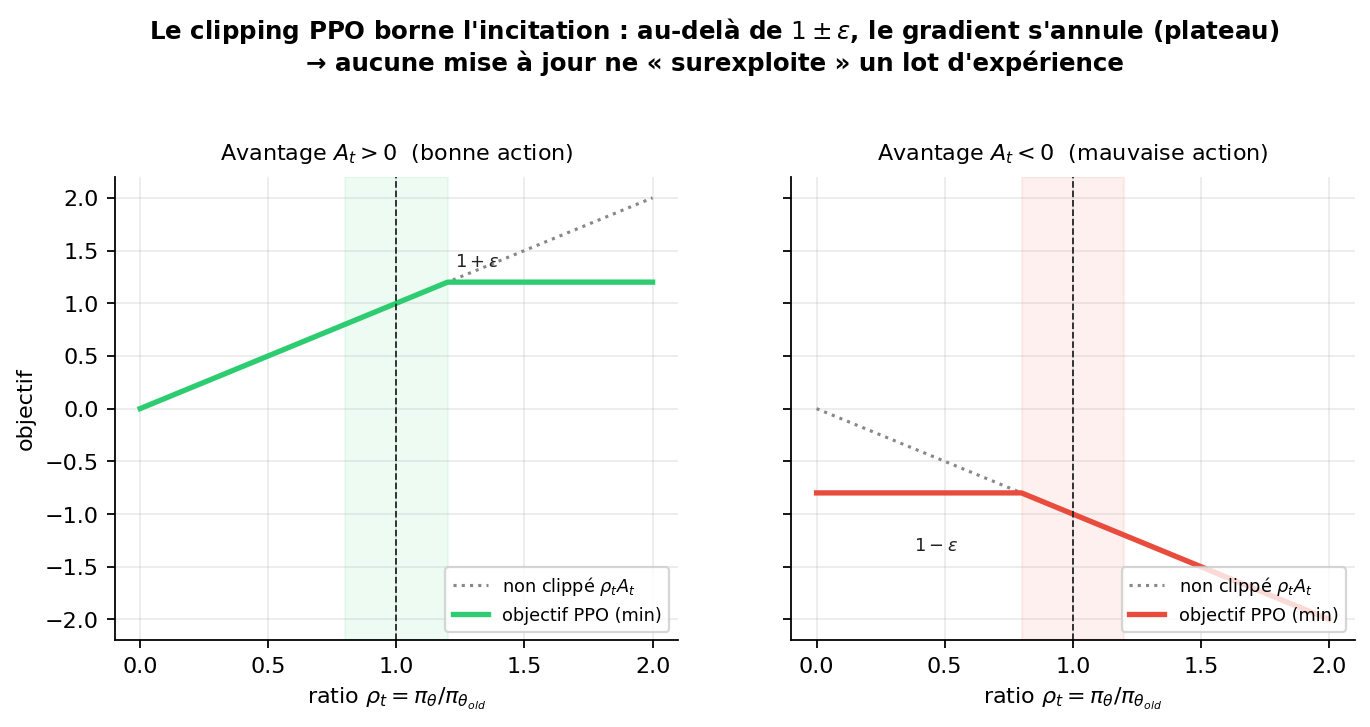
\includegraphics[width=\textwidth]{fig_ppo_clip.png}
\caption{Le mécanisme central de PPO. L'objectif suit le gain espéré $\rho_t A_t$ tant
que la nouvelle politique reste proche de l'ancienne ($\rho_t \in [1-\epsilon,
1+\epsilon]$), puis \emph{plafonne} : au-delà, augmenter encore la probabilité de
l'action n'apporte plus rien au gradient. On ne peut donc jamais « tout miser » sur un
lot d'expérience chanceux --- exactement la garde-fou qu'exigent des données aussi
bruitées que des rendements.}
\label{fig:ppoclip}
\end{figure}

Trois rouages qu'il faut savoir expliquer :
\begin{itemize}[itemsep=2pt]
  \item \textbf{fonction de valeur} : un second réseau estime $V(s_t)$, « ce que cet
        état devrait rapporter en moyenne » ; l'avantage $A_t$ mesure ce que l'action a
        rapporté \emph{au-delà} de cette attente --- c'est lui qui dit au gradient quoi
        renforcer ;
  \item \textbf{bonus d'entropie} (coefficient $0{,}05$) : un petit terme qui récompense
        le fait de garder des probabilités d'action diversifiées ; sans lui, la
        politique se fige prématurément sur une action (typiquement « toujours Hold »
        ou « toujours Long ») avant d'avoir exploré les alternatives ;
  \item \textbf{normalisation des observations} (\code{VecNormalize}) : pendant
        l'entraînement, moyenne et variance \emph{glissantes} de chaque composante de
        l'observation sont maintenues, et les observations sont standardisées à la
        volée. Distinct du scaler des features (section~\ref{sec:features}) : il couvre
        aussi position et PnL, et ses statistiques doivent être \emph{sauvegardées avec
        le modèle} --- un modèle nourri d'observations brutes à l'évaluation produit du
        non-sens, comme je l'ai appris à mes dépens (section~\ref{sec:iter2}).
\end{itemize}

\subsection{Trois choix de conception --- et les alternatives écartées}

\begin{itemize}[itemsep=3pt]
  \item \textbf{PPO plutôt que DQN ou SAC.} Trois familles existaient : les méthodes
        \emph{value-based} (DQN : apprendre $Q(s,a)$ puis agir gloutonnement ---
        réputées instables sur des récompenses bruitées et non stationnaires, et
        sujettes à la surestimation des valeurs) ; les \emph{policy gradients
        on-policy} (A2C, PPO : optimiser directement la politique sur l'expérience
        fraîche) ; les méthodes \emph{off-policy continues} (SAC, TD3 : efficaces en
        données mais pour actions continues et plus délicates à régler). PPO gagne pour
        moi par sa \textbf{stabilité} (le clipping borne chaque mise à jour --- crucial
        quand le signal est du bruit à 95\,\%), son support natif des actions
        discrètes, et son statut de standard reproductible dans Stable-Baselines3.
  \item \textbf{Actions discrètes (4) plutôt que continues.} Le tout-ou-rien simplifie
        l'apprentissage et rend chaque action \emph{économiquement lisible} (long,
        cash, short) --- au prix d'une gestion du risque binaire, limite documentée en
        section~\ref{sec:limites} ; le passage à une position continue $[-1, 1]$ est le
        levier suivant.
  \item \textbf{Données journalières.} Compromis entre le bruit (l'intraday exigerait
        de modéliser la microstructure que mon simulateur ignore) et la quantité
        d'expérience (le mensuel n'offrirait que $\sim$150 décisions par actif). Au
        pas journalier, 13 ans $\times$ 5 actifs $\approx$ 16\,000 jours de décision.
\end{itemize}

\subsection{Single-agent, multi-actifs, multi-agents : ne pas confondre}
\label{sec:marl}

Trois notions que je tiens à distinguer précisément, parce que la confusion est
fréquente (et que mon propre vocabulaire de projet peut la créer) :

\begin{itemize}[itemsep=3pt]
  \item \textbf{Single-agent, mono-actif} : un décideur, un actif (mon modèle
        « Single », entraîné sur AAPL seul). L'environnement est stationnaire du point
        de vue de l'agent --- au sens où ses propres actions n'influencent pas les prix.
  \item \textbf{Single-agent, multi-actifs} : c'est mon modèle « Multi (5 tickers) » :
        \emph{un seul} agent, entraîné sur les données de cinq actifs (chaque épisode se
        déroule sur un actif, tiré au hasard). Ce n'est PAS du multi-agents : c'est de la
        \emph{régularisation par diversité des données} --- pour être bon sur AAPL, MSFT,
        GOOGL, SPY et TSLA à la fois, il faut des règles générales, pas une trajectoire
        apprise par c\oe ur.
  \item \textbf{Multi-agents (MARL)} : plusieurs politiques \emph{apprennent
        simultanément} et interagissent. La difficulté fondamentale : du point de vue de
        chaque agent, l'environnement devient \emph{non stationnaire}, puisque les autres
        agents changent en apprenant --- les garanties de convergence du RL classique
        sautent. La réponse standard est le CTDE (\emph{centralized training,
        decentralized execution}) : un critique centralisé qui voit tout pendant
        l'entraînement, des politiques décentralisées à l'exécution (MAPPO, MADDPG).
        C'est la phase suivante de ma roadmap : ajouter un \emph{adversaire de marché}
        qui apprend à créer les scénarios les plus défavorables (chocs de liquidité,
        pics de volatilité) --- de l'\emph{adversarial training} pour forcer la
        robustesse, précisément la faiblesse que le walk-forward va révéler
        (section~\ref{sec:wf}).
\end{itemize}

% ============================================================
\section{Features : le pont avec l'économétrie}
\label{sec:features}
% ============================================================

Chaque feature que je donne à l'agent répond à un problème identifié en économétrie des
séries temporelles.

\begin{table}[H]
\centering\small
\begin{tabular}{@{}lp{5.6cm}p{6.2cm}@{}}
\toprule
\textbf{Feature} & \textbf{Définition} & \textbf{Notion d'économétrie associée} \\
\midrule
\code{log\_returns} & $r_t = \ln(P_t/P_{t-1})$ &
Les prix sont $I(1)$ (non stationnaires, cf.\ test ADF) : je travaille sur la série
différenciée, stationnaire en moyenne, comme pour toute modélisation ARMA. \\
\addlinespace
\code{volatility} & écart-type glissant de $r_t$ sur 20 jours &
Estimateur naïf de $\sigma_t$ : proxy du \emph{volatility clustering} modélisé par
GARCH(1,1), $\sigma_t^2 = \omega + \alpha \varepsilon_{t-1}^2 + \beta \sigma_{t-1}^2$
(Engle, Bollerslev). L'agent observe le régime de volatilité sans estimer le modèle. \\
\addlinespace
\code{rsi} & oscillateur borné $[0,1]$ sur 14 jours &
Signal de sur-achat/sur-vente : pari de \emph{retour à la moyenne} local --- l'esprit
d'un processus d'Ornstein-Uhlenbeck, $dX_t = \kappa(\mu - X_t)\,dt + \sigma\,dW_t$,
qui rappelle la variable vers sa moyenne $\mu$ à vitesse $\kappa$, sans son estimation
paramétrique. \\
\addlinespace
\code{macd\_norm} & $(\text{EMA}_{12}-\text{EMA}_{26})/\text{EMA}_{26}$ &
Détection de tendance par différence de moyennes mobiles exponentielles ---
un filtre linéaire de la série des prix. \\
\addlinespace
\code{momentum\_5} & rendement sur 5 jours &
Anomalie \emph{momentum} (Jegadeesh \& Titman, 1993) : autocorrélation positive des
rendements à moyen terme, une des violations les plus documentées de l'efficience
faible. \\
\bottomrule
\end{tabular}
\caption{Correspondance features $\leftrightarrow$ économétrie.}
\end{table}

\paragraph{Le biais de look-ahead, version machine learning.}
En économétrie, on n'évalue jamais un modèle sur l'échantillon qui a servi à l'estimer.
Ici, l'équivalent se niche dans un détail : la \emph{normalisation}. Le
\code{RobustScaler} (centrage médiane, réduction par écart interquartile --- robuste aux
queues épaisses des rendements) est \textbf{fitté sur le train uniquement}, puis appliqué
tel quel à la validation et au test. Le fitter sur tout l'échantillon reviendrait à
injecter dans les observations de 2015 des statistiques calculées avec les données de
2022 : de l'information future. Un test unitaire verrouille ce point en comparant les
paramètres du scaler à ceux d'un scaler fitté manuellement sur le train seul.

\begin{figure}[H]
\centering
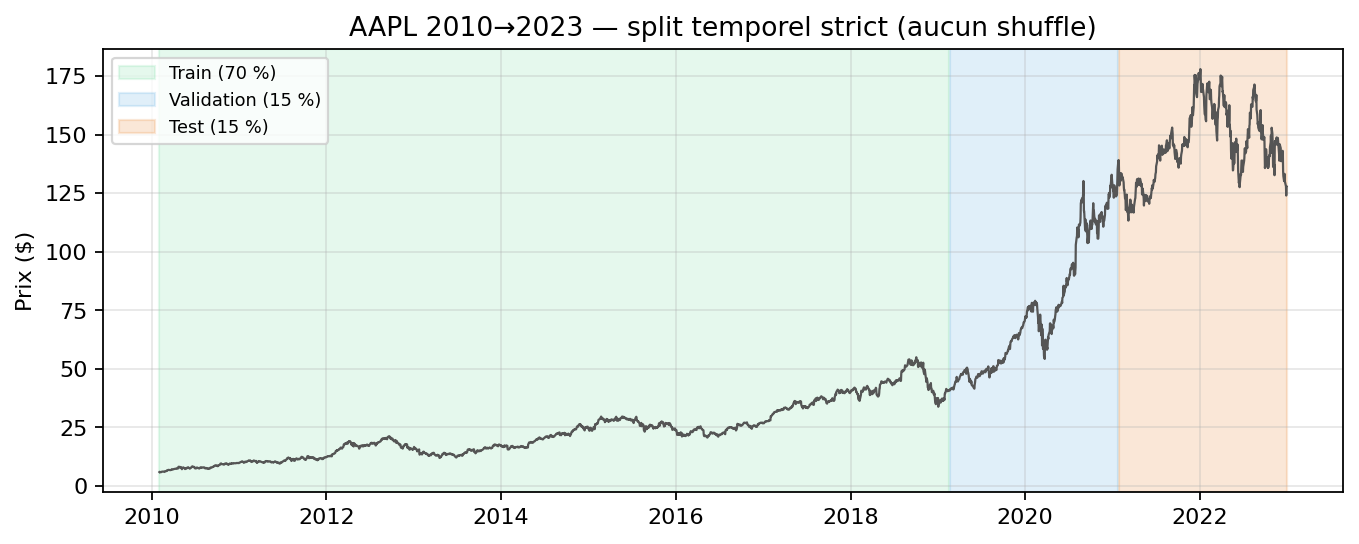
\includegraphics[width=\textwidth]{fig_data_splits.png}
\caption{Split temporel strict 70/15/15 sur AAPL 2010$\to$2023. Le train couvre
plusieurs cycles (2011, 2015, 2018), la validation contient le krach COVID et sa
reprise, le test enchaîne bull 2021 et bear 2022. C'est l'équivalent de l'évaluation
out-of-sample d'un modèle économétrique.}
\label{fig:splits}
\end{figure}

\paragraph{Zoom : le retour à la moyenne et le processus d'Ornstein-Uhlenbeck.}
C'est le modèle canonique du retour à la moyenne en temps continu :
\[
dX_t = \kappa\,(\mu - X_t)\,dt + \sigma\,dW_t ,
\]
où $\mu$ est le niveau de long terme, $\kappa > 0$ la \emph{vitesse de rappel} (plus
$\kappa$ est grand, plus vite tout écart se résorbe) et $\sigma\,dW_t$ le choc brownien.
Deux quantités à savoir manier : la \textbf{demi-vie} d'un écart, $t_{1/2} = \ln 2 /
\kappa$ (« en combien de jours la moitié de l'écart à $\mu$ est-elle effacée ? »), et le
lien direct avec l'économétrie : \emph{discrétisé, un OU est exactement un AR(1)},
$X_{t+1} = \mu(1-\varphi) + \varphi X_t + \varepsilon_t$ avec $\varphi =
e^{-\kappa \Delta t}$ --- on estime donc $\kappa$ par une simple régression MCO de
$X_{t+1}$ sur $X_t$ (dérivation complète en annexe~\ref{app:ou}). Dans ce projet, je
n'estime pas d'OU : le RSI en est le cousin non paramétrique (un oscillateur borné qui
signale les écarts extrêmes susceptibles de se résorber). Mais le cadre OU est celui
que j'utiliserais pour trader un \emph{spread} de paires cointégrées --- le projet
suivant sur ma liste --- et c'est le vocabulaire attendu en entretien dès qu'on dit
« mean reversion ».

\begin{figure}[H]
\centering
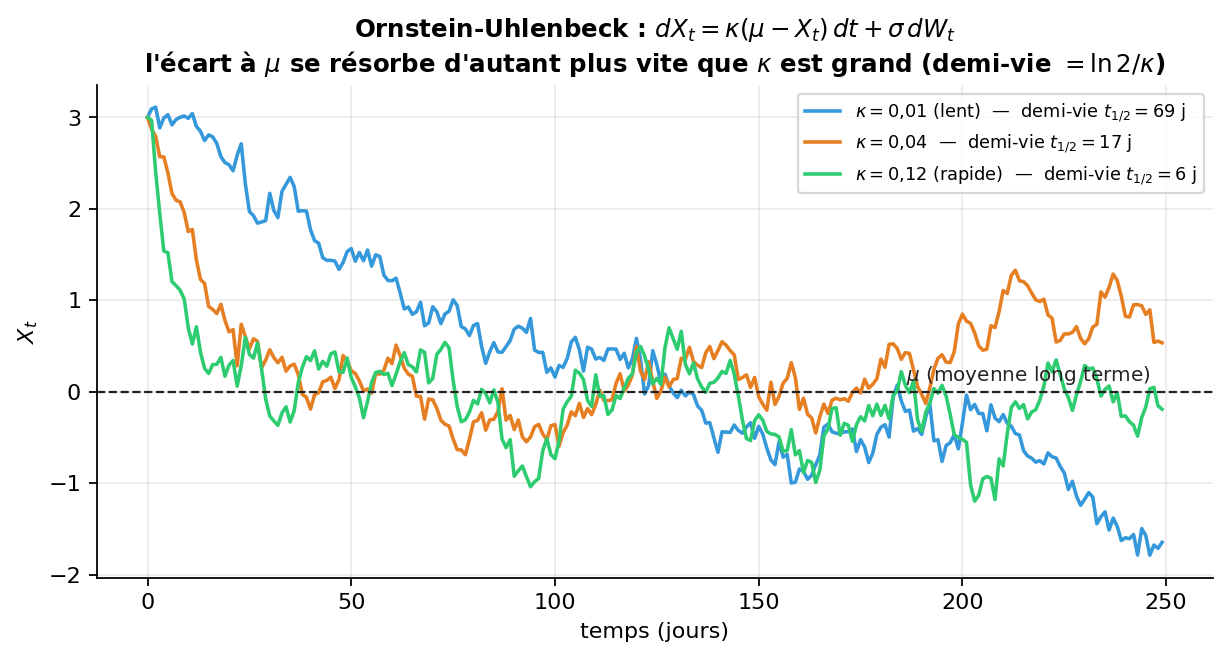
\includegraphics[width=0.82\textwidth]{fig_ou_process.png}
\caption{Trois processus d'Ornstein-Uhlenbeck partant du même écart initial. Plus la
vitesse de rappel $\kappa$ est grande, plus vite la trajectoire revient vers $\mu$ ---
la \emph{demi-vie} $\ln 2/\kappa$ quantifie ce « temps de retour ». C'est l'objet qu'un
stratège stat-arb estime sur le spread d'une paire avant de décider s'il vaut la peine
d'être tradé.}
\label{fig:ou}
\end{figure}

\begin{figure}[H]
\centering
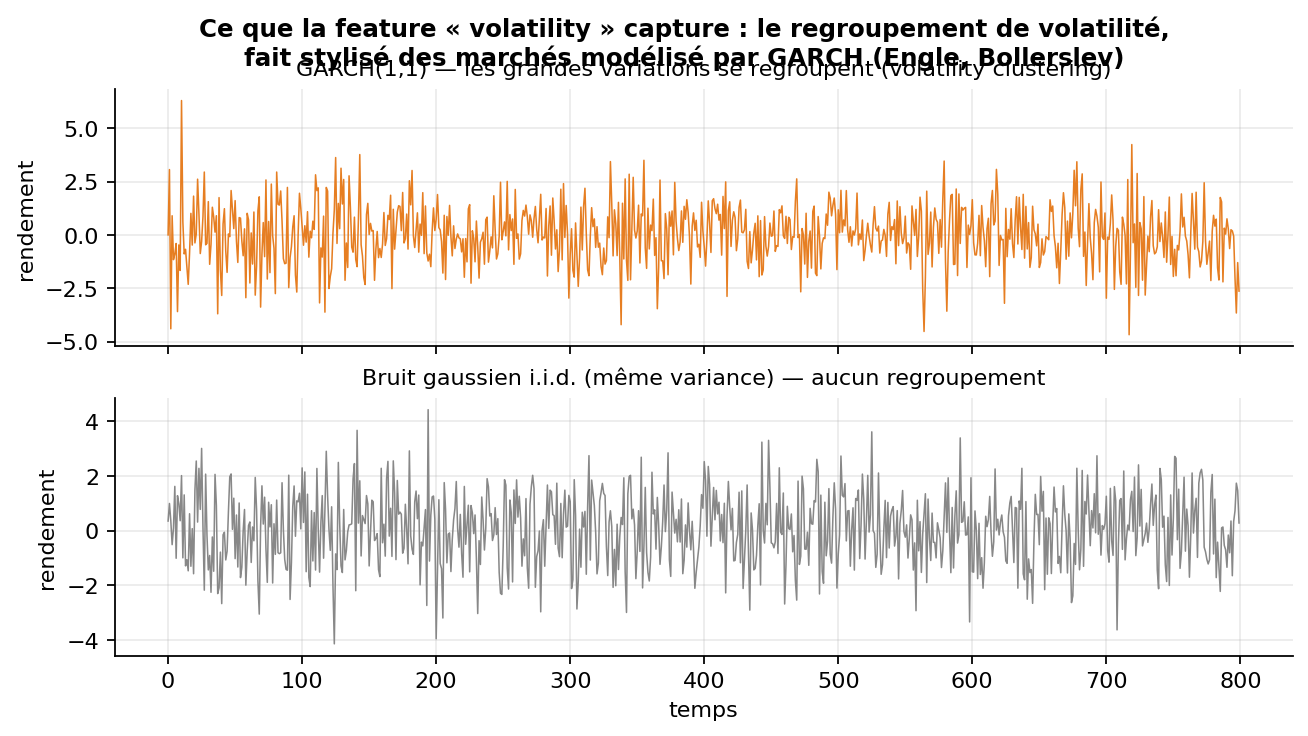
\includegraphics[width=0.92\textwidth]{fig_vol_clustering.png}
\caption{Ce que la feature \code{volatility} donne à voir à l'agent. En haut, un
GARCH(1,1) : les grandes variations s'agglutinent (une journée agitée en annonce une
autre) --- le \emph{volatility clustering}, fait stylisé omniprésent des marchés. En
bas, un bruit gaussien de même variance : aucune structure. La rolling-std de 20 jours
est un estimateur naïf de l'état de volatilité du haut.}
\label{fig:vol}
\end{figure}
\label{sec:reward}
% ============================================================

\subsection{Pourquoi ma récompense est un alpha de Jensen par pas de temps}

Mon premier réflexe avait été une récompense de type Sharpe par pas. Symptôme observé :
l'agent devenait « toujours long ». Diagnostic : comme le marché monte en moyenne sur la
période, \emph{suivre le marché} suffit à collecter du rendement --- la récompense ne
distinguait pas « profiter du marché » de « battre le marché ». J'ai donc changé la
cible : à chaque pas,
\[
r_t = \underbrace{\left(\frac{V_t - V_{t-1}}{V_{t-1}} - \frac{P_t - P_{t-1}}{P_{t-1}}\right)}_{\text{alpha du pas } t}
\times\, 100
\;-\; \text{pénalité de frais} \;-\; 0{,}05 \times \text{drawdown},
\]
où $V_t$ est la valeur du portefeuille et $P_t$ le prix. Le premier terme est un
\textbf{alpha de Jensen} dans le cas particulier $\beta = 1$, $R_f = 0$ :
\[
\alpha_J = R_p - \big[R_f + \beta\,(R_m - R_f)\big] \;\xrightarrow{\;\beta=1,\; R_f=0\;}\; R_p - R_m .
\]
Être long quand ça monte ne rapporte plus rien (alpha $\approx 0$) ; être cash ou short
quand ça baisse rapporte ; rater une hausse coûte. L'agent est payé pour \emph{timer},
pas pour \emph{suivre}. Le facteur $\times 100$ est une mise à l'échelle : PPO apprend
bien avec des récompenses d'ordre de grandeur $\sim 1$, alors qu'un return journalier
brut ($\sim 0{,}01$) donnerait un signal de gradient trop faible.

Les deux pénalités sont des outils de gestion classiques : les \textbf{frais}
($0{,}1\,\%$ par transaction, débités du portefeuille \emph{et} pénalisés dans la
récompense) découragent l'overtrading ; la pénalité de \textbf{drawdown} introduit une
aversion au risque asymétrique, complétée par un \emph{kill-switch} : tout épisode dont
le drawdown dépasse $25\,\%$ s'arrête --- l'équivalent d'un stop-loss de mandat.

\subsection{Métriques d'évaluation}

Toutes viennent du cours de gestion de portefeuille :
\begin{itemize}[itemsep=2pt]
  \item \textbf{Sharpe} $= \frac{\bar{r}}{\hat\sigma}\sqrt{252}$ : rendement par unité de
        risque total (critère moyenne-variance de Markowitz) ;
  \item \textbf{Sortino} : idem avec l'écart-type des seuls rendements négatifs
        (semi-variance) --- on ne pénalise pas la volatilité haussière ;
  \item \textbf{Max drawdown} : perte maximale depuis un pic, le risque « vécu » ;
  \item \textbf{Calmar} $=$ rendement annualisé $/$ max drawdown ;
  \item \textbf{CVaR$_{95}$} (Expected Shortfall)
        $= \mathbb{E}[r \mid r \le \text{VaR}_{95}]$, où la VaR$_{95}$ est simplement le
        quantile à $5\,\%$ des rendements journaliers (« le seuil de perte dépassé un
        jour sur vingt »). La CVaR répond à la question suivante : \emph{quand} ce seuil
        est franchi, combien perd-on en moyenne ? Contrairement à la VaR, c'est une
        mesure cohérente (sous-additive), celle de la réglementation bancaire récente.
\end{itemize}

% ============================================================
\section{Chronologie : ce qui ne marchait pas, ce que j'ai changé}
\label{sec:evolution}
% ============================================================

C'est le c\oe ur du rapport. Chaque itération suit le même schéma : \emph{symptôme
observé $\to$ diagnostic $\to$ pourquoi c'est grave financièrement $\to$ décision $\to$
résultat mesuré $\to$ ce que ça ouvre}.

\subsection{Point de départ}

Deux modèles PPO entraînés sur 2018--2023 (un mono-actif AAPL, un multi-actifs),
récompense alpha, observations normalisées par \code{VecNormalize}. Mon évaluation
d'alors donnait : Single battant le B\&H sur 3 tirages sur 5 (alpha moyen
$+8{,}5\,\% \pm 10{,}2$), Multi négatif ($-4{,}7\,\%$, 0/5).

Trois symptômes me gênaient : (i) une variance énorme entre tirages ($\pm 10$ à
15 points --- comment conclure quoi que ce soit ?), (ii) un alpha d'entraînement de
plusieurs milliers de pourcents (personne ne croit ça : mémorisation), (iii) un Multi
« toujours long », alors que sa raison d'être était justement de généraliser.
\emph{Avant de toucher au modèle, j'ai décidé de fiabiliser tout ce qui produit les
chiffres.}

\subsection{Itération 1 --- des tests, parce qu'un simulateur faux rend tout faux}

En finance simulée, un test ne vérifie pas que « le code tourne » : il vérifie que
\emph{l'économie du simulateur est juste}. J'ai écrit une suite de tests qui fixe des
vérités comptables : un aller-retour long à prix constant doit coûter exactement
$(1-c)^2$ du capital ; un short doit gagner quand le prix baisse ; le kill-switch doit
se déclencher au bon seuil ; la normalisation ne doit rien voir du futur.

\textbf{Résultat} : les tests ont immédiatement trouvé une asymétrie --- \ko{les frais
d'ouverture d'un short n'étaient pas débités du portefeuille} (ils réduisaient
seulement la taille de position), contrairement au long. Un simulateur qui sous-facture
le short gonfle mécaniquement toute stratégie qui shorte : exactement le genre de biais
qui fabrique de faux alphas. Corrigé, verrouillé par un test de symétrie.

\emph{Ce que ça ouvre : avec un simulateur fiable, je peux maintenant regarder si mes
chiffres d'évaluation, eux, sont crédibles.}

\subsection{Itération 2 --- mon protocole d'évaluation mentait}
\label{sec:iter2}

Trois défauts faussaient les \emph{conclusions}, indépendamment de la qualité des
modèles :

\begin{enumerate}[itemsep=3pt]
  \item \ko{Observations non normalisées à l'évaluation.} Le modèle est entraîné sur
        des observations standardisées ; deux scripts prédisaient sur observations
        \emph{brutes}. C'est comme estimer une régression sur variables
        centrées-réduites puis prédire sur variables en niveau : les sorties n'ont
        aucun sens.
  \item \ko{Frais d'évaluation $\ne$ frais d'entraînement} ($0{,}2\,\%$ vs $0{,}1\,\%$) :
        j'évaluais l'agent dans un monde deux fois plus coûteux que celui où il avait
        appris à trader.
  \item \ko{Évaluation sur fenêtres aléatoires uniquement}, d'où la variance de
        $\pm 15$ points. Pire : un épisode arrêté par le kill-switch se termine
        \emph{par construction} à son point bas, et était comparé à un B\&H calculé sur
        une fenêtre différente --- des alphas incomparables entre modèles.
\end{enumerate}

\textbf{Décision} : un protocole de référence \ok{déterministe sur le split complet}
(départ fixe, politique déterministe, reproductible au centime) ; si le kill-switch se
déclenche, la stratégie est réputée liquidée et \ok{reste en cash jusqu'à la fin de la
fenêtre} --- tous les modèles et le B\&H sont ainsi comparés sur le même horizon. Les
fenêtres aléatoires deviennent une mesure \emph{complémentaire} de robustesse au point
d'entrée.

\emph{Ce que ça ouvre : des chiffres enfin stables --- et donc la possibilité de voir
qu'il restait un vrai problème de données.}

\subsection{Itération 3 --- plus de cycles de marché}

Symptôme : mon test d'origine (avril--décembre 2022) était un bear pur. Interprétation
financière : sur une telle période, un agent simplement \emph{peureux} paraît génial ---
biais de période classique du backtesting. Décision : réentraîner sur 2010$\to$2023
($2{,}6\times$ plus de données, plusieurs corrections dans le train, validation
contenant le COVID) avec un test 2021--2022 qui enchaîne hausse \emph{et} baisse.

\emph{Ce que ça ouvre : un cadre assez propre pour que le dernier symptôme --- le Multi
toujours décevant --- ne puisse plus s'expliquer que par une vraie cause.}

\subsection{Itération 4 --- le bug décisif : ma validation était corrompue}
\label{sec:bug}

Symptôme : après réentraînement, le Multi restait mauvais (alpha test négatif, biais
long), \emph{et} les logs d'entraînement montraient des drawdowns de validation de 45 à
50\,\% --- physiquement impossibles avec un kill-switch à 25\,\%.

Diagnostic : le pipeline multi-actifs concatène les données des cinq tickers. Un
identifiant de segment garantissait que les épisodes d'\emph{entraînement} ne
franchissent pas la frontière entre deux actifs\ldots{} mais pas ceux de la
\emph{validation}. Un épisode de validation pouvait donc passer du dernier jour de
GOOGL ($\sim$1\,000\,\$) au premier jour de SPY ($\sim$300\,\$) : un krach fictif de
$-70\,\%$ en un jour.

Pourquoi c'est grave : c'est précisément sur cette validation que l'\code{EvalCallback}
choisit le \emph{best model} conservé à la fin. \textbf{Je sélectionnais mon meilleur
modèle sur du bruit} --- l'équivalent économétrique d'un critère de choix de modèle
calculé sur un échantillon pollué.

\textbf{Décision et résultat} : une ligne de correction (segments sur les trois splits),
un réentraînement --- le Multi passe à \ok{$+27{,}5\,\%$ d'alpha} sur le test, avec un
alpha positif sur \ok{5/5 actifs} (figure~\ref{fig:cross}) et une répartition d'actions
enfin équilibrée. La leçon que je retiens : \emph{la sélection de modèle vaut ce que
vaut le signal de validation}.

\paragraph{La preuve propre : une ablation contrôlée.}
Le tableau~\ref{tab:evolution} a une faiblesse méthodologique que je préfère lever
moi-même : entre « départ » et « final », j'ai changé plusieurs choses (dates,
protocole, frais du short, bug de validation) --- c'est un \emph{confondage}, on ne
sait pas quelle cause a produit quel effet. J'ai donc mené l'expérience contrôlée :
réentraîner le Multi \textbf{en ne réintroduisant que le bug} (validation sans
segments), tout le reste strictement identique (données 2010--2023, seed, 800\,000
pas, protocole d'évaluation final).

\begin{table}[H]
\centering\small
\begin{tabular}{@{}lcc@{}}
\toprule
\textbf{Multi, toutes choses égales par ailleurs} & \textbf{Validation corrompue} & \textbf{Validation propre} \\
\midrule
Alpha test AAPL & \ko{$-2{,}4\,\%$} & \ok{$+27{,}5\,\%$} \\
Actifs à alpha positif & 3/5 & \ok{5/5} \\
Alpha cross-actifs moyen & $+10{,}4\,\%$ & \ok{$+17{,}2\,\%$} \\
\bottomrule
\end{tabular}
\caption{Ablation contrôlée du bug de validation : effet causal isolé $\approx +30$
points d'alpha sur AAPL. Détail du modèle corrompu : TSLA $+37\,\%$, GOOGL $+20{,}5\,\%$,
MSFT $+5{,}9\,\%$, AAPL $-2{,}4\,\%$, SPY $-8{,}8\,\%$.}
\label{tab:ablationbug}
\end{table}

Le détail est aussi instructif que la moyenne : le modèle sélectionné sur une
validation bruitée n'est pas \emph{uniformément} mauvais --- il est \emph{erratique}
(excellent sur TSLA, négatif sur AAPL et SPY). C'est exactement ce que prédit la
théorie : sélectionner sur du bruit revient à tirer un checkpoint \emph{au hasard}
parmi les versions du réseau --- une loterie, dont on gagne certains tickets. La
validation propre ne rend pas le modèle plus intelligent ; elle rend sa sélection
\emph{systématique} au lieu d'aléatoire.

\emph{Ce que ça ouvre : des résultats crédibles sur UN split. Reste la question qu'un
professionnel poserait immédiatement : et sur les autres périodes ?
(section~\ref{sec:wf}).}

\subsection{Récapitulatif chiffré}

\begin{table}[H]
\centering\small
\begin{tabular}{@{}lccc@{}}
\toprule
 & \textbf{Départ} & \textbf{Après itérations 1--4} & \\
\textbf{Indicateur (test set)} & \small (2018-23, protocole v0) & \small (2010-23, protocole final) & \\
\midrule
Alpha Single & $+8{,}5\,\% \pm 10{,}2$ & $+19{,}2\,\%$ & \ok{$\uparrow$} \\
Alpha Multi & $-4{,}7\,\% \pm 2{,}8$ & $+27{,}5\,\%$ & \ok{$\uparrow$} \\
Fenêtres où Single $>$ B\&H & 3/5 & 5/5 & \ok{$\uparrow$} \\
Fenêtres où Multi $>$ B\&H & 0/5 & 5/5 & \ok{$\uparrow$} \\
Actifs à alpha positif (Multi) & 1/5 & 5/5 & \ok{$\uparrow$} \\
Répartition des actions (Multi) & biais long & équilibrée (short 23\,\%) & \ok{$\uparrow$} \\
\bottomrule
\end{tabular}
\caption{Avant/après. Les protocoles diffèrent entre colonnes \emph{parce que corriger
le protocole fait partie des améliorations} ; chaque chiffre est mesuré avec le
protocole en vigueur à son étape (section~\ref{sec:iter2}). L'effet du bug de
validation \emph{seul}, toutes choses égales par ailleurs, est isolé par l'ablation
contrôlée du tableau~\ref{tab:ablationbug}.}
\label{tab:evolution}
\end{table}

\begin{figure}[H]
\centering
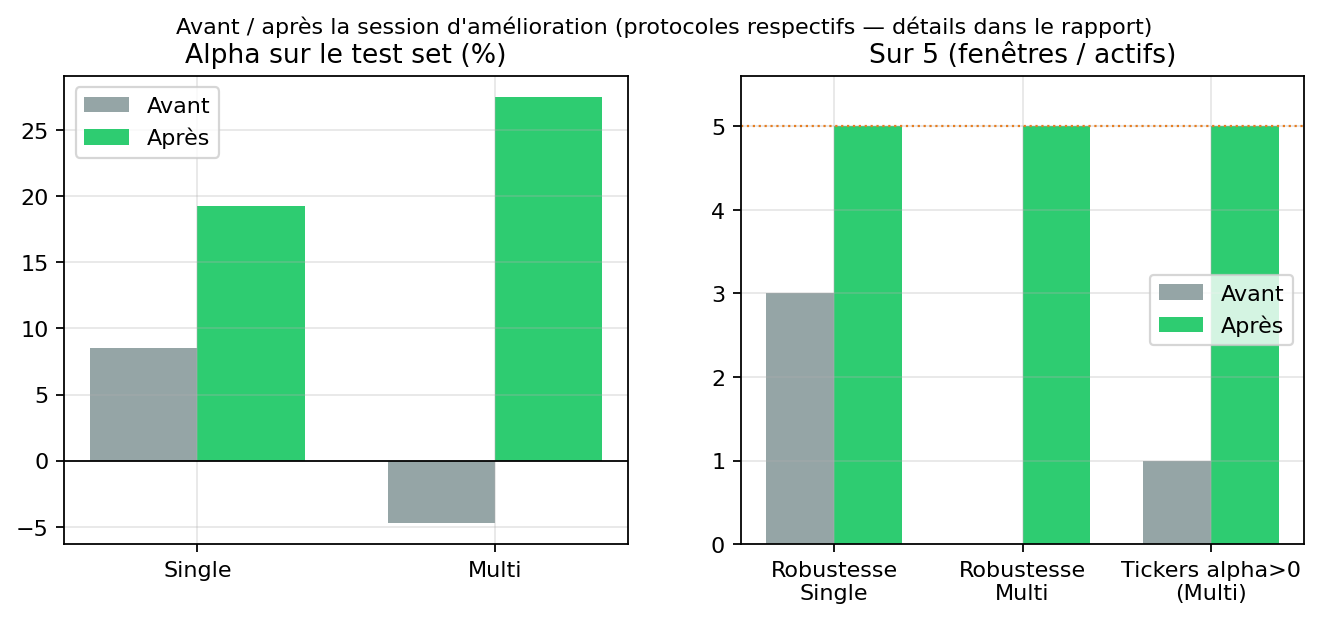
\includegraphics[width=\textwidth]{fig_evolution.png}
\caption{Synthèse graphique du tableau~\ref{tab:evolution}.}
\label{fig:evolution}
\end{figure}

% ============================================================
\section{Résultats sur le split de référence}
\label{sec:resultats}
% ============================================================

\subsection{Test AAPL, février 2021 $\to$ décembre 2022}

\begin{table}[H]
\centering\small
\begin{tabular}{@{}lrrrrrrr@{}}
\toprule
\textbf{Modèle} & \textbf{Return} & \textbf{Alpha} & \textbf{MaxDD} & \textbf{Sharpe}
& \textbf{Sortino} & \textbf{Calmar} & \textbf{CVaR$_{95}$} \\
\midrule
Single (AAPL) & $+15{,}5\,\%$ & $+19{,}2\,\%$ & $26{,}2\,\%$ & $0{,}44$ & $0{,}57$ & $0{,}30$ & $-3{,}4\,\%$ \\
Multi (5 actifs) & $\mathbf{+23{,}8\,\%}$ & $\mathbf{+27{,}5\,\%}$ & $25{,}2\,\%$ & $\mathbf{0{,}57}$ & $\mathbf{0{,}77}$ & $\mathbf{0{,}47}$ & $-3{,}7\,\%$ \\
\midrule
Buy \& Hold (réf.) & $-3{,}7\,\%$ & --- & $30{,}3\,\%$ & --- & --- & --- & --- \\
\bottomrule
\end{tabular}
\caption{Évaluation déterministe sur le split complet. Robustesse : les deux modèles
battent le B\&H sur 5/5 sous-fenêtres aléatoires (Single $+9{,}0\,\%\pm4{,}9$,
Multi $+8{,}1\,\%\pm3{,}1$).}
\label{tab:final}
\end{table}

\paragraph{Mise à jour (Acte 3, section~\ref{sec:seeds}).} L'alpha \emph{mono-actif} de
ce tableau porte une incertitude de $\pm 21$ points selon le seed d'entraînement --- le
$+27{,}5\,\%$ vient du haut de la distribution. La statistique robuste est la moyenne
cross-actifs : \textbf{$+14{,}5\,\% \pm 6{,}5$, positive pour 5 seeds sur 5} sur cette
fenêtre de test.

\begin{figure}[H]
\centering
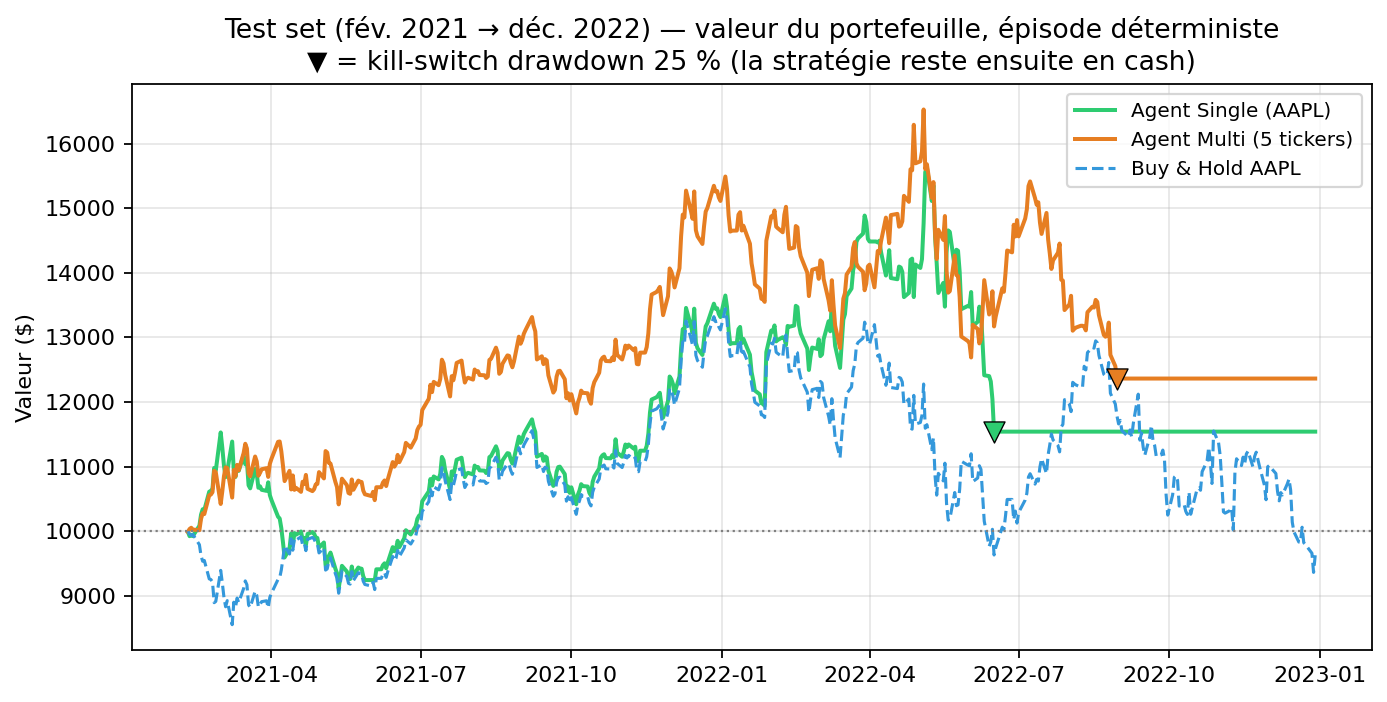
\includegraphics[width=\textwidth]{fig_equity_test.png}
\caption{Valeur du portefeuille sur le test. Lecture : les agents suivent la hausse de
2021 (le Multi la surperforme), encaissent une partie du retournement de 2022, puis le
kill-switch les sort du marché ($\blacktriangledown$) --- ils finissent en cash pendant
que le B\&H replonge. Une part importante de l'alpha vient de cette
\emph{non-exposition} finale : vraie décision de gestion du risque, mais il faut le
dire --- et la section~\ref{sec:wf} montrera ce que ça implique.}
\label{fig:equity}
\end{figure}

\begin{figure}[H]
\centering
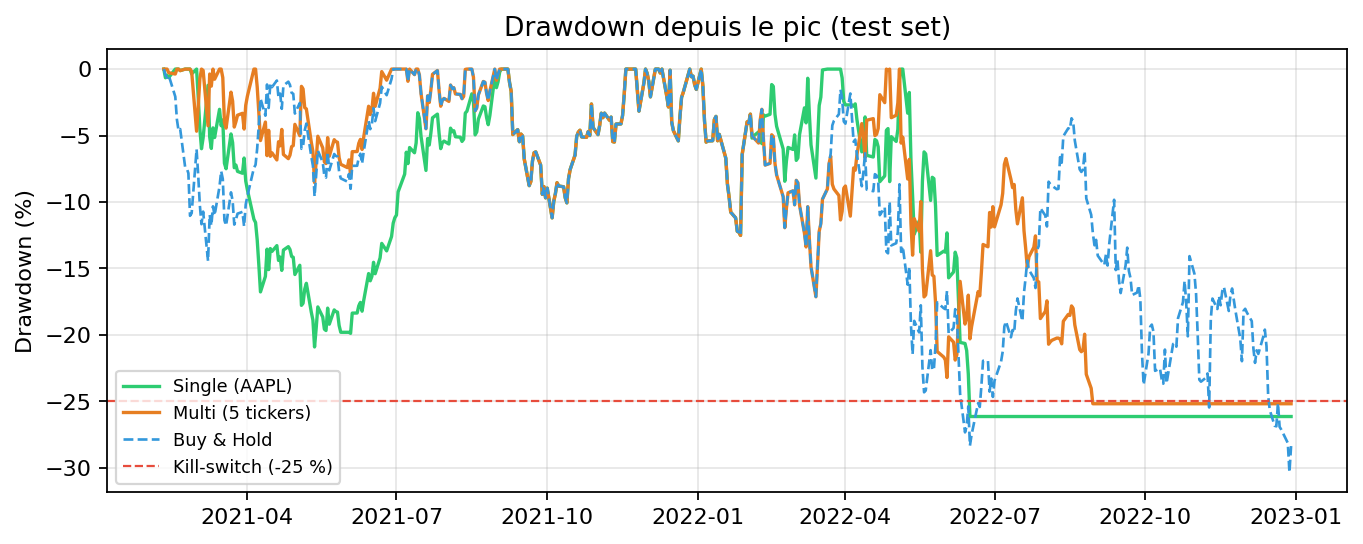
\includegraphics[width=\textwidth]{fig_drawdown_test.png}
\caption{Drawdown depuis le pic : les agents restent bornés par le kill-switch à
$-25\,\%$ quand le B\&H dépasse $-30\,\%$.}
\label{fig:dd}
\end{figure}

\subsection{Généralisation cross-actifs}

\begin{figure}[H]
\centering
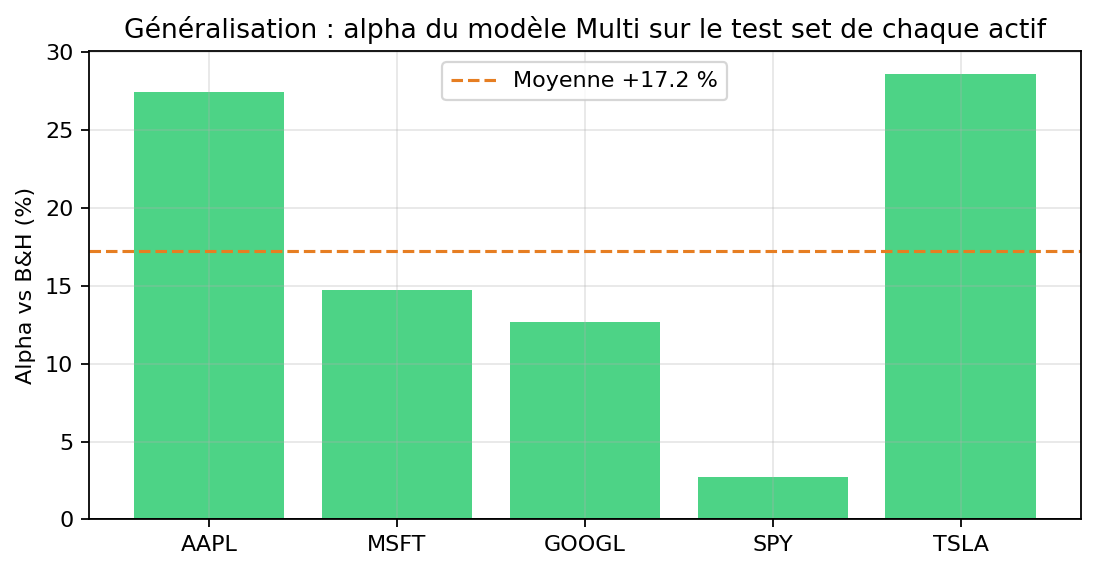
\includegraphics[width=0.85\textwidth]{fig_cross_ticker.png}
\caption{Alpha du Multi sur le test de chaque actif : positif sur 5/5, moyenne
$+17{,}2\,\%$. Un modèle qui aurait mémorisé AAPL ne transférerait pas sur TSLA
($+28{,}6\,\%$) ni GOOGL ($+12{,}7\,\%$).}
\label{fig:cross}
\end{figure}

\begin{figure}[H]
\centering
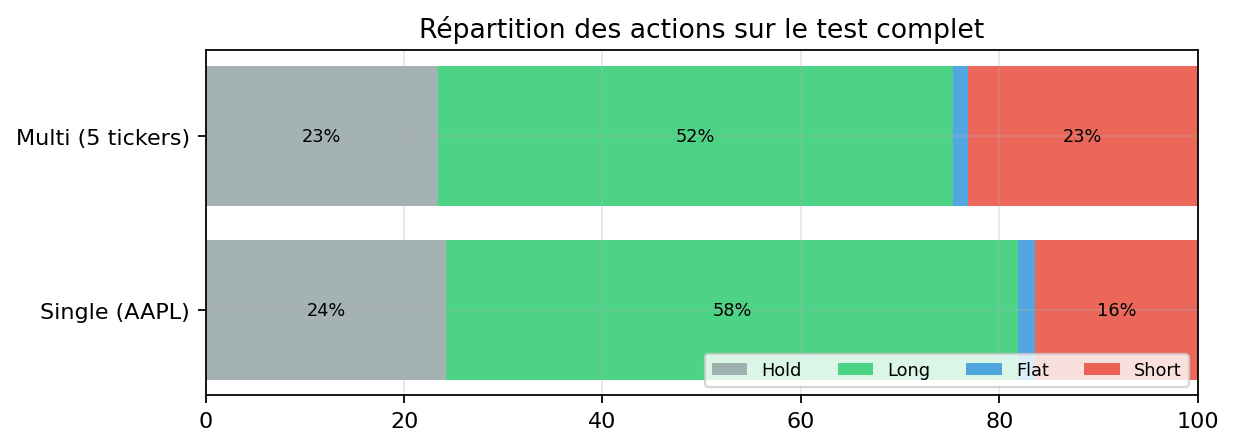
\includegraphics[width=0.8\textwidth]{fig_actions.png}
\caption{Répartition des actions sur le test complet. Le Multi est équilibré (short
$23\,\%$ du temps) là où sa version pré-correction était longue en quasi-permanence.}
\label{fig:actions}
\end{figure}

À ce stade, j'avais un résultat solide \emph{sur une période}. Mais je savais --- pour
l'avoir écrit moi-même dans les limites --- qu'un backtest unique est \emph{un tirage},
pas une distribution. La suite s'imposait d'elle-même.

% ============================================================
\section{Du backtest unique au walk-forward}
\label{sec:wf}
% ============================================================

\subsection{Pourquoi c'était la priorité (et pas la diffusion ou le MARL)}

Mes lectures me tiraient vers l'avant : politiques par diffusion, génération de
scénarios synthétiques, multi-agents. Mais je me suis imposé trois questions avant de
choisir :

\begin{enumerate}[itemsep=2pt]
  \item \emph{Ma conclusion actuelle est-elle fiable ?} Non --- elle repose sur une
        seule période de test, choisie par moi.
  \item \emph{Qu'est-ce qu'un professionnel me demanderait en premier ?} « Montre-moi la
        stabilité temporelle » --- pas « ajoute un modèle de diffusion ».
  \item \emph{Que vaut une sophistication bâtie sur une évaluation fragile ?} Rien : je
        ne saurais même pas dire si elle améliore quoi que ce soit.
\end{enumerate}

Décision : consolider la fondation d'abord. Le \emph{walk-forward} est le standard du
backtesting sérieux : on réentraîne le modèle en ne voyant que le passé, on le teste
sur l'année suivante, on avance, on répète. C'est la généralisation dynamique du
principe out-of-sample de l'économétrie : non pas \emph{un} échantillon de test, mais
une \emph{séquence} d'échantillons de test, chacun prédit par un modèle qui ne connaît
que son passé.

\subsection{Protocole}

Fenêtre \emph{croissante ancrée} (anchored) : pour chaque année de test
$Y \in \{2018, \ldots, 2022\}$, j'entraîne sur $[2010, Y)$ (dont les derniers 15\,\%
servent de validation pour la sélection du best model), puis j'évalue sur l'année $Y$
--- 100\,\% out-of-sample --- pour chacun des cinq actifs. Soit 5 réentraînements
complets et $5 \times 5 = 25$ cellules année$\times$actif. Deux limites assumées :
400\,000 pas d'entraînement par fold (contre 800\,000 pour le modèle de référence,
pour un temps de calcul raisonnable), et des folds anciens qui voient moins d'histoire.

\begin{figure}[H]
\centering
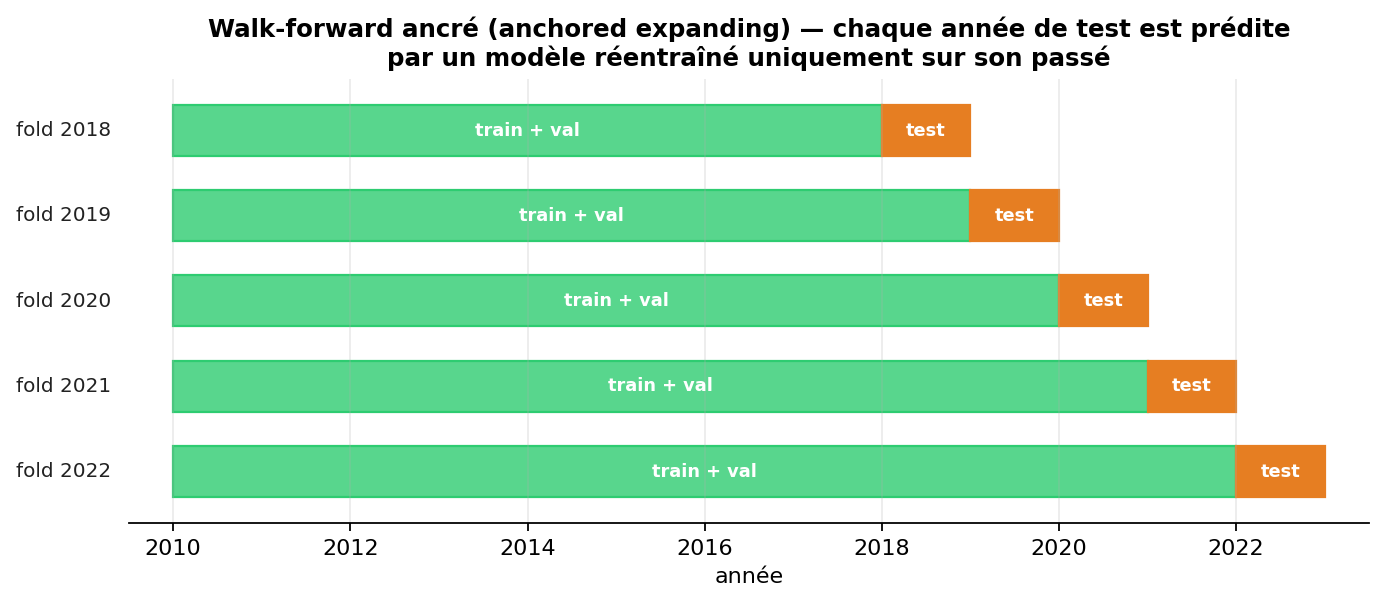
\includegraphics[width=0.9\textwidth]{fig_walkforward_schema.png}
\caption{Le protocole en image. Chaque ligne est un fold : le modèle n'apprend que sur
le passé (vert, ancré à 2010) et n'est jugé que sur l'année suivante (orange), jamais
vue. En avançant fold après fold, on obtient une \emph{séquence} de tests
out-of-sample au lieu d'un seul --- la généralisation dynamique du principe de
l'échantillon de test en économétrie.}
\label{fig:wfschema}
\end{figure}

\subsection{Ce que j'avais prédit --- et ce qui s'est passé}

Avant de lancer, j'ai noté ma prédiction : \emph{l'alpha moyen serait nettement plus
faible que le $+27{,}5\,\%$ du split unique --- 2022 étant l'année rêvée pour un agent
défensif --- mais je m'attendais à une médiane positive.} La première moitié s'est
vérifiée. La seconde non : médiane $-2{,}0\,\%$, 48\,\% de cellules positives. Et c'est
la moitié fausse qui m'a le plus appris.

\begin{table}[H]
\centering\small
\begin{tabular}{@{}lrrrl@{}}
\toprule
\textbf{Année OOS} & \textbf{Agent (moy.)} & \textbf{B\&H (moy.)} & \textbf{Alpha} & \textbf{Régime} \\
\midrule
2018 & $+5{,}2\,\%$  & $-4{,}0\,\%$   & \ok{$+9{,}2\,\%$}   & année baissière \\
2019 & $+21{,}2\,\%$ & $+42{,}2\,\%$  & \ko{$-21{,}0\,\%$}  & bull soutenu \\
2020 & $-3{,}0\,\%$  & $+143{,}3\,\%$ & \ko{$-146{,}4\,\%$} & krach puis rebond violent \\
2021 & $+32{,}2\,\%$ & $+43{,}3\,\%$  & \ko{$-11{,}1\,\%$}  & bull \\
2022 & $+6{,}2\,\%$  & $-31{,}4\,\%$  & \ok{$+37{,}6\,\%$}  & bear \\
\midrule
\multicolumn{5}{l}{\small Agrégat : alpha moyen $-26{,}3\,\%$ (médiane $-2{,}0\,\%$,
écart-type $106\,\%$), 48\,\% de cellules $>0$.} \\
\bottomrule
\end{tabular}
\caption{Walk-forward, moyennes par fold sur les 5 actifs. La moyenne est écrasée par
2020 --- en particulier la cellule TSLA (B\&H $+576\,\%$, alpha $-514\,\%$) : rater UNE
année de rebond extrême coûte plus que tout ce que la défense rapporte ailleurs.}
\label{tab:wf}
\end{table}

\begin{figure}[H]
\centering
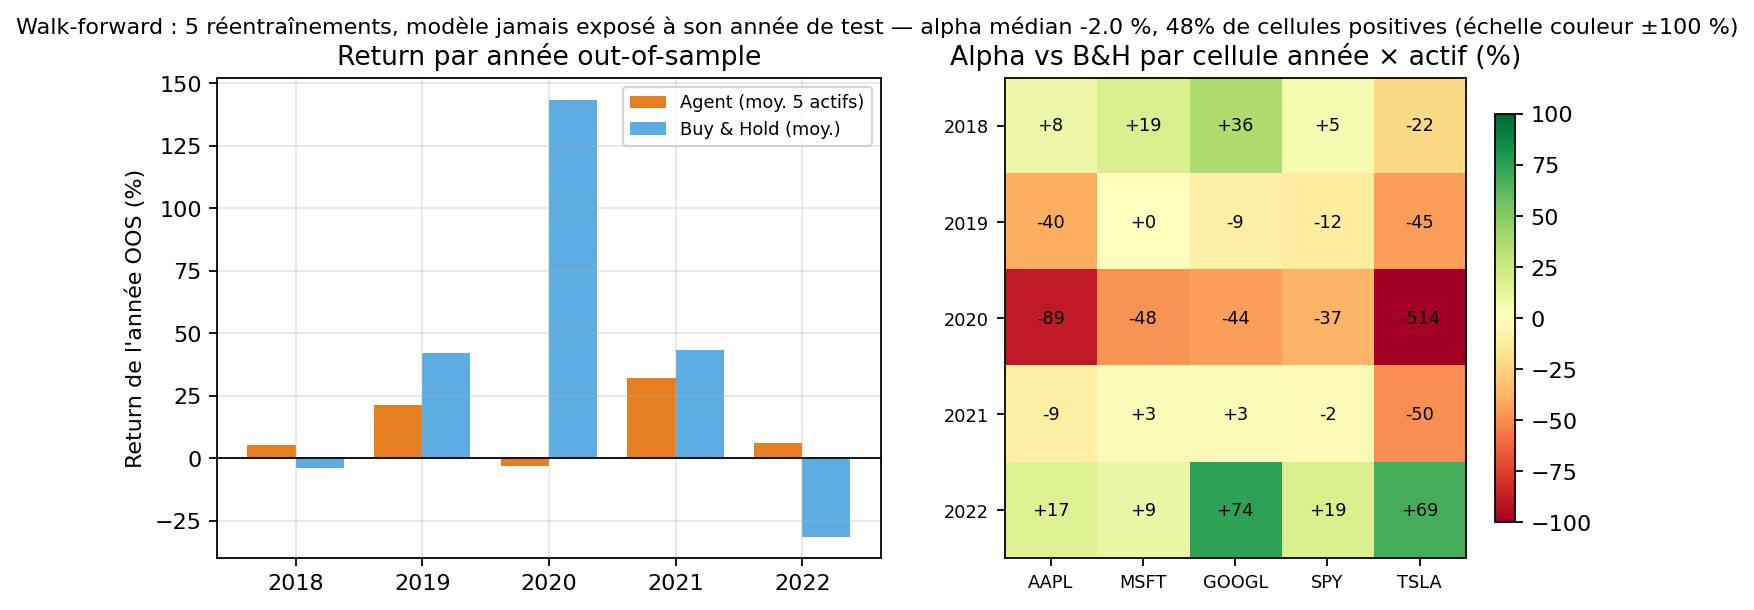
\includegraphics[width=\textwidth]{fig_walk_forward.png}
\caption{À gauche : return absolu de l'agent (orange) vs B\&H (bleu) par année
out-of-sample. À droite : grille des 25 alphas (couleur tronquée à $\pm 100\,\%$).
Le motif est net : vert sur les lignes 2018 et 2022 (marchés baissiers), rouge sur
2019--2021 (marchés haussiers).}
\label{fig:wf}
\end{figure}

\subsection{Interprétation financière : un profil, pas un alpha universel}

\begin{itemize}[itemsep=3pt]
  \item \textbf{L'agent est un profil défensif régime-dépendant.} Alpha nettement
        positif les années baissières (2018 : $+9\,\%$ ; 2022 : $+38\,\%$), proche de
        zéro à négatif en marché haussier, catastrophique --- \emph{relativement au
        B\&H} --- dans un rebond violent (2020 : stoppé dans le krach, il reste
        défensif pendant que le marché fait $+143\,\%$).
  \item \textbf{En absolu, le tableau est différent} : rendement positif 4 années sur 5,
        et $+5$ à $+6\,\%$ les deux années où le B\&H perd. Comme brique
        \emph{absolute return} défensive dans une allocation, le profil est cohérent ;
        comme stratégie « qui bat le marché », non.
  \item \textbf{Mon $+27{,}5\,\%$ du split unique n'était donc pas faux, mais
        partiel} : 2021--2022 contient précisément le régime où ce profil excelle.
        C'est la démonstration empirique, sur mon propre projet, du biais de période
        --- je l'avais énoncé en théorie à l'itération 3, le walk-forward le quantifie.
  \item \textbf{Moyenne vs médiane} : l'écart ($-26\,\%$ vs $-2\,\%$) vient d'une queue
        gauche épaisse (TSLA 2020). Réflexe d'économètre : sur des distributions
        asymétriques à outliers, la médiane est la statistique robuste --- mais ici
        l'outlier n'est pas une erreur de mesure, c'est un vrai scénario de marché :
        le coût d'opportunité des rebonds fait partie du risque de la stratégie.
\end{itemize}

\subsection{Ce que ça ouvre}

Le diagnostic « défensif partout, y compris quand il ne faudrait pas » pointe vers une
cause précise : l'agent n'observe rien qui lui permette de \emph{distinguer les
régimes} --- il applique la même prudence dans un krach durable et dans un rebond en V.
Trois pistes, par ordre de priorité que je me fixe :
\begin{enumerate}[itemsep=2pt]
  \item \textbf{features de régime} (tendance longue, distance au plus-haut d'un an,
        vitesse de reprise) --- l'esprit des modèles à changement de régime de type
        \emph{Markov-switching} (Hamilton, 1989), vus en économétrie : les paramètres
        du processus sautent entre quelques états latents (bull, bear) pilotés par une
        chaîne de Markov cachée, et on infère l'état courant à partir des données.
        \emph{Piste testée depuis, et falsifiée --- voir la section~\ref{sec:regime}} ;
  \item \textbf{position continue} (action $\in [-1, 1]$) au lieu du tout-ou-rien, pour
        que la défense soit graduelle et non binaire ;
  \item \textbf{adversarial training multi-agents} (section~\ref{sec:marl}) et
        génération de scénarios par diffusion --- ma roadmap initiale --- qui ne
        prennent leur sens que maintenant : j'ai enfin un protocole capable de mesurer
        si elles améliorent la robustesse.
\end{enumerate}

% ============================================================
\section{Stress-tests : les questions qu'un desk poserait}
\label{sec:stress}
% ============================================================

Pour juger mon propre travail, je me suis mis dans la peau d'un trader qui lit ce
rapport. Ses deux premières questions sont prévisibles --- alors autant y répondre avec
des mesures plutôt que des arguments. Aucun réentraînement ici : je stresse les
\emph{hypothèses d'exécution et de risque}, à politique fixée
(\code{evaluate.stress\_report()}).

\subsection{« Ton alpha survit-il à des frais réalistes ? »}

Mes modèles sont entraînés avec $0{,}10\,\%$ de frais par trade. J'évalue les mêmes
politiques sous une grille de coûts --- une façon de proxyser spread, slippage et
(partiellement) le coût d'emprunt des shorts que mon simulateur ne modélise pas :

\begin{table}[H]
\centering\small
\begin{tabular}{@{}lrrrrr@{}}
\toprule
\textbf{Alpha (test)} & \textbf{0\,bp} & \textbf{5\,bp} & \textbf{10\,bp} & \textbf{20\,bp} & \textbf{30\,bp} \\
\midrule
Single (AAPL), 259 trades & $+24{,}9\,\%$ & $+22{,}0\,\%$ & $+19{,}2\,\%$ & $+13{,}8\,\%$ & $+8{,}7\,\%$ \\
Multi (5 actifs), 301 trades & $+28{,}7\,\%$ & $+28{,}0\,\%$ & $+27{,}5\,\%$ & $+25{,}7\,\%$ & $\mathbf{+23{,}7\,\%}$ \\
\bottomrule
\end{tabular}
\caption{Sensibilité de l'alpha au niveau de frais par trade (test AAPL 2021--2022).
1\,bp (point de base) $= 0{,}01\,\%$ ; 10\,bp = niveau d'entraînement.}
\label{tab:fees}
\end{table}

Réponse : \ok{l'edge du Multi n'est pas un artefact de coûts} --- il ne perd que 5
points d'alpha entre 0 et 30\,bp, soit trois fois le niveau de frais auquel il a été
entraîné. Le Single, lui, se dégrade nettement ($-16$ points sur la grille) : son
avantage est plus fragile à l'exécution.

\subsection{« Que reste-t-il si j'enlève ton kill-switch ? »}

La figure~\ref{fig:equity} suggérait qu'une part importante de l'alpha 2022 venait de la
sortie du marché sur stop. Je l'ai quantifiée : mêmes politiques, drawdown libre (seul
le stop de quasi-ruine à $5\,\%$ du capital subsiste).

\begin{table}[H]
\centering\small
\begin{tabular}{@{}lrrrr@{}}
\toprule
\textbf{Sans kill-switch} & \textbf{Return} & \textbf{Alpha} & \textbf{MaxDD} & \textbf{Contribution du stop} \\
\midrule
Single (AAPL) & $-5{,}4\,\%$ & \ko{$-1{,}7\,\%$} & $44{,}9\,\%$ & $+21{,}0$ points \\
Multi (5 actifs) & $+1{,}4\,\%$ & \ok{$+5{,}1\,\%$} & $40{,}4\,\%$ & $+22{,}3$ points \\
\bottomrule
\end{tabular}
\caption{Ablation du kill-switch sur le test. « Contribution du stop » = alpha avec stop
$-$ alpha sans stop (la règle inclut la non-réexposition jusqu'à la fin de la fenêtre).}
\label{tab:ablation}
\end{table}

La réponse est la découverte la plus importante de ce projet après le walk-forward :
\textbf{environ 21 points d'alpha sur 2022 viennent de la règle de stop, pas du timing
quotidien}. Sans elle, le Single ne bat plus le marché du tout ($-1{,}7\,\%$) ; le Multi
conserve un alpha de décision modeste mais réel ($+5{,}1\,\%$), en subissant un drawdown
de $40\,\%$.

Interprétation en langage de desk : je distingue désormais \emph{l'alpha de signal}
(les décisions jour par jour --- faible mais positif pour le Multi) de \emph{l'alpha de
règle de risque} (couper l'exposition sur drawdown --- majoritaire ici). Ce n'est pas
disqualifiant : le stop fait partie de la stratégie que j'ai conçue, et c'est lui qui
borne le MaxDD à $25\,\%$ quand le marché fait $-30\,\%$. Mais vendre ce système comme
du « market timing par RL » serait faux : c'est \emph{une discipline de risque
systématique, aidée par un signal RL modeste}. Cette phrase résume honnêtement le
projet.

\subsection{Les questions restantes --- et celle qui a depuis reçu sa mesure}

\begin{itemize}[itemsep=2pt]
  \item \emph{Sensibilité au seed d'entraînement} : mesurée depuis à
        l'Acte~3 (section~\ref{sec:seeds}) --- $\pm 21$ points sur un actif isolé,
        $\pm 6{,}5$ sur la moyenne cross-actifs, positive pour 5 seeds sur 5.
  \item \emph{Coût d'emprunt des shorts} : non modélisé explicitement (le stress de
        frais le capture partiellement) ; sur des titres chers à emprunter, l'alpha
        short de 2022 serait rogné.
  \item \emph{Exécution au cours de clôture} : pas d'écart d'exécution intrajournalier
        ni d'impact de marché.
\end{itemize}


% ============================================================
\section{Acte 3 : attaquer la dépendance de régime}
\label{sec:acte3}
% ============================================================

Le diagnostic est posé (sections~\ref{sec:wf} et~\ref{sec:stress}) : profil défensif
régime-dépendant, alpha majoritairement porté par la règle de stop. La suite logique
saute aux yeux --- « rendre l'agent conscient des régimes ». Mais avant de tester le
moindre traitement, il me manque une chose : \textbf{une barre d'erreur}. Le RL profond
est notoirement sensible au hasard d'initialisation (poids du réseau, ordre
d'exploration) ; tant que je ne connais pas la dispersion de mes résultats d'un seed à
l'autre, je ne peux pas distinguer une amélioration réelle d'un tirage chanceux. D'où le
plan de cet acte : (1) mesurer le bruit, (2) tester le traitement, (3) conclure
\emph{hors bruit}.

\subsection{D'abord la barre d'erreur : cinq seeds}
\label{sec:seeds}

\paragraph{Protocole.} Quatre réentraînements complets du Multi, strictement identiques
au modèle de référence (données 2010--2023, 800\,000 pas, validation propre), en ne
changeant que le seed --- 7, 123, 777, 2024, plus le 42 existant. Un détail qui aurait
tout invalidé : le seed était \emph{codé en dur} dans l'appel à PPO ; sans le
paramétrer d'abord, mes « cinq entraînements » auraient été cinq copies du même tirage.

\paragraph{Ce que j'avais prédit.} Une dispersion non triviale mais un signe stable ---
alpha AAPL positif pour au moins 4 seeds sur 5.

\paragraph{Résultat : prédiction fausse, leçon meilleure.}

\begin{table}[H]
\centering\small
\begin{tabular}{@{}lrrc@{}}
\toprule
\textbf{Seed} & \textbf{Alpha AAPL} & \textbf{Alpha cross-actifs (moy.)} & \textbf{Actifs $>0$} \\
\midrule
7    & $+43{,}6\,\%$ & $+16{,}5\,\%$ & 4/5 \\
42 (référence) & $+27{,}5\,\%$ & $+17{,}2\,\%$ & 5/5 \\
123  & $-5{,}1\,\%$  & $+10{,}6\,\%$ & 3/5 \\
777  & $-2{,}3\,\%$  & $+23{,}7\,\%$ & 3/5 \\
2024 & $-11{,}2\,\%$ & $+4{,}3\,\%$  & 3/5 \\
\midrule
Moyenne $\pm$ écart-type & $+10{,}5\,\% \pm 21{,}3$ & \ok{$+14{,}5\,\% \pm 6{,}5$} & --- \\
\bottomrule
\end{tabular}
\caption{Robustesse au seed d'entraînement (test 2021--2022, protocole identique au
tableau~\ref{tab:final}). L'alpha cross-actifs est positif pour \ok{5 seeds sur 5}.}
\label{tab:seeds}
\end{table}

L'alpha \emph{sur AAPL seul} est une loterie : de $-11$ à $+44\,\%$ selon le seed,
positif 2 fois sur 5 --- mon $+27{,}5\,\%$ de référence vient du haut de cette
distribution. Mais la moyenne \emph{sur les cinq actifs} est remarquablement plus
stable et \ok{positive pour tous les seeds}.

\begin{figure}[H]
\centering
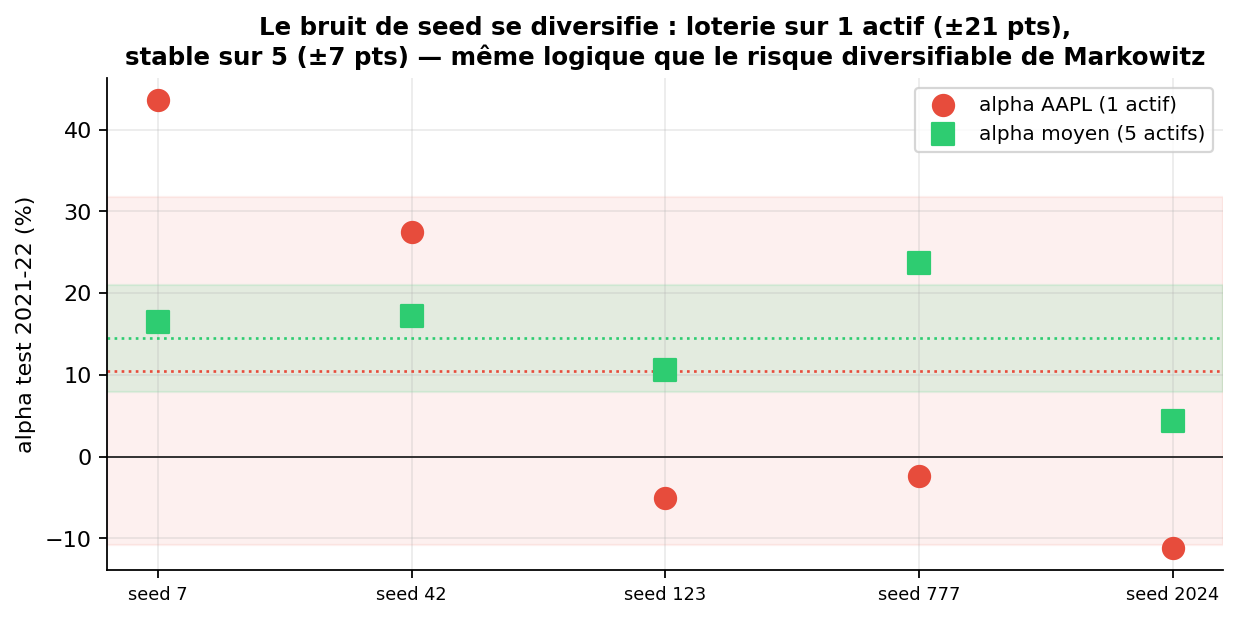
\includegraphics[width=0.82\textwidth]{fig_seed_dispersion.png}
\caption{La leçon de l'acte, en une image. Chaque colonne est un seed d'entraînement.
Les points rouges (alpha d'un seul actif) sont dispersés sur $\pm 21$ points ; les
carrés verts (moyenne sur cinq actifs) tiennent dans une bande de $\pm 6{,}5$. Le bruit
d'initialisation, largement idiosyncratique par actif, se \emph{diversifie} en
moyennant --- la même mécanique que le risque spécifique dans un portefeuille.}
\label{fig:seeds}
\end{figure}

\paragraph{Pourquoi cet écart ? La théorie du portefeuille, encore.} Le bruit de seed
frappe chaque couple (seed, actif) de manière largement idiosyncratique ; en moyennant
sur cinq actifs, il se diversifie --- exactement comme le risque spécifique d'un titre
dans un portefeuille de Markowitz. Deux conséquences que j'applique immédiatement :
\begin{itemize}[itemsep=2pt]
  \item \textbf{le chiffre défendable n'est pas l'alpha d'un actif, c'est la moyenne
        cross-actifs} : $+14{,}5\,\% \pm 6{,}5$ sur cette fenêtre de test --- les
        sections vivantes du rapport sont mises à jour en conséquence ;
  \item \textbf{toute expérience future se juge contre la bande $\pm 6{,}5$ points} :
        en dessous, c'est du bruit, quel que soit l'enthousiasme.
\end{itemize}

\subsection{Le traitement : des features de régime --- et son échec instructif}
\label{sec:regime}

\paragraph{Hypothèse et protocole.} Le diagnostic du walk-forward disait : l'agent ne
distingue pas un krach durable d'un rebond en V. Le traitement le plus direct consiste
à \emph{lui montrer le régime}. J'ai ajouté deux features long-terme à l'observation
($52 \to 72$ entrées) : \code{dist\_high\_252}, la position par rapport au plus-haut
d'un an (le drawdown de l'actif lui-même --- proche de zéro en bull, $-30\,\%$ en
krach), et \code{trend\_200}, la position par rapport à la moyenne mobile 200 jours
(LE proxy de régime des praticiens). Tout le reste est identique --- données
2010--2023, configuration, seed 42 --- et le candidat s'entraîne dans un dossier
séparé : promotion uniquement s'il bat la bande de bruit de la
section~\ref{sec:seeds}.

\paragraph{Ce que j'avais prédit.} Amélioration du fold 2020 (le pire : $-146\,\%$)
sans dégradation de 2022.

\paragraph{Résultat : faux sur les deux volets.}

\begin{table}[H]
\centering\small
\begin{tabular}{@{}lrr@{}}
\toprule
\textbf{Alpha moyen (5 actifs)} & \textbf{Baseline (obs 52)} & \textbf{+ régime (obs 72)} \\
\midrule
2018 (bear)            & $+9{,}2\,\%$   & $+30{,}3\,\%$\footnotemark \\
2019 (bull)            & $-21{,}0\,\%$  & $-5{,}7\,\%$ \\
2020 (krach + rebond)  & $-146{,}4\,\%$ & \ko{$-162{,}5\,\%$} \\
2021 (bull)            & $-11{,}1\,\%$  & \ko{$-51{,}7\,\%$} \\
2022 (bear)            & $+37{,}6\,\%$  & \ko{$+17{,}2\,\%$} \\
\midrule
Walk-forward : médiane / cellules $>0$ & $-2{,}0\,\%$ / 48\,\% & $-2{,}9\,\%$ / 36\,\% \\
Test 2021-22 : cross-actifs / positifs & $+17{,}2\,\%$ / 5 sur 5 & $+11{,}6\,\%$ / 2 sur 5 \\
\bottomrule
\end{tabular}
\caption{Baseline contre candidat « régime », même seed, même protocole.}
\label{tab:regime}
\end{table}
\footnotetext{Tiré par une seule cellule (TSLA 2018 : $+145{,}6\,\%$) --- davantage un
ticket de loterie qu'un signe de clairvoyance, cf.\ la dispersion mesurée en
section~\ref{sec:seeds}.}

\paragraph{Verdict : pas de promotion.} Sur la fenêtre de test, le candidat tombe dans
la bande de bruit, du mauvais côté ($+11{,}6\,\%$, 2 actifs positifs sur 5). Sur le
walk-forward, la dégradation est cohérente précisément là où le traitement devait
agir : 2020 \emph{empire}, 2021 s'effondre, et même 2022 --- la force du profil ---
recule. Une seule seed, certes ; mais quand toutes les années clés bougent dans le même
sens, l'explication « bruit » ne tient plus.

\paragraph{Pourquoi cet échec est un bon résultat.} Mon hypothèse d'« underfitting de
représentation » est falsifiée dans sa version naïve : \textbf{voir le régime ne suffit
pas à l'exploiter}. La récompense de l'agent (alpha par pas, pénalité de drawdown,
kill-switch) ne valorise pas différemment la prudence selon le régime --- ajouter des
colonnes à l'observation ne change pas les \emph{incitations}, et l'espace d'entrée
élargi offre surtout plus de latitude pour sur-apprendre. La contrainte active n'était
pas l'information mais la structure de la récompense et l'action tout-ou-rien. En
économiste, je devrais reconnaître le schéma : les agents répondent aux incitations,
pas aux informations qu'on leur affiche.

\subsection{Bilan de l'acte}

Trois acquis, dont deux méthodologiques :
\begin{enumerate}[itemsep=2pt]
  \item \textbf{la revendication robuste du projet} : alpha cross-actifs
        $+14{,}5\,\% \pm 6{,}5$ sur le test 2021-22, positif pour 5 seeds sur 5
        (l'alpha mono-actif, lui, est une loterie à $\pm 21$ points) ;
  \item \textbf{une barre d'erreur permanente} : toute expérience future se juge
        contre la bande inter-seeds, pas contre un chiffre unique ;
  \item \textbf{une direction falsifiée et une nouvelle priorité} : le prochain levier
        n'est pas l'observation mais la récompense et le dimensionnement de position
        (action continue, aversion au risque dépendante du régime).
\end{enumerate}


% ============================================================
\section{Overfitting, underfitting, régimes : le diagnostic complet}
% ============================================================

\paragraph{L'overfitting se voit sur le train.} Le Single réalise sur son propre train
un alpha de l'ordre de $+16\,500\,\%$ : de la \textbf{mémorisation} de trajectoire,
l'équivalent d'un $R^2$ in-sample de $0{,}999$. Ce chiffre ne mesure rien d'autre que
la capacité du réseau à apprendre par c\oe ur --- ce qui compte est out-of-sample.

\paragraph{Mes remèdes.} Entraînement multi-actifs (régularisation par les données) ;
\emph{early stopping} --- on conserve la version du réseau qui maximise la performance
de \emph{validation}, pas la dernière : si la fin de l'entraînement sur-apprend, on ne
la paie pas (d'où le caractère critique du bug de la section~\ref{sec:bug}) ; réseau
volontairement petit ; clipping PPO ; bonus d'entropie ; plus d'années de données.

\paragraph{Et l'underfitting ?} C'est le défaut symétrique : un modèle trop simple pour
capter le signal disponible, reconnaissable à de mauvaises performances \emph{partout,
y compris sur le train}. Mon alpha d'entraînement délirant prouve que la capacité ne
manque pas. En revanche, le walk-forward révèle un underfitting plus subtil : un
underfitting de \emph{représentation}. Mes cinq features ne contiennent tout simplement
pas l'information « dans quel régime de marché sommes-nous ? » --- aucun réseau, aussi
gros soit-il, ne peut apprendre à distinguer un krach durable d'un rebond en V s'il ne
voit que dix jours de features court-terme. Le problème n'est pas la capacité du
modèle, c'est ce que je lui donne à regarder.

\paragraph{La distinction que le walk-forward m'a forcé à faire.} Avant, je risquais de
tout appeler « overfitting ». Maintenant je sépare trois choses :
\begin{itemize}[itemsep=2pt]
  \item \textbf{mémorisation} (train $\gg$ test) : présente, contenue par les remèdes
        ci-dessus, et visible ;
  \item \textbf{biais de période} (un test favorable au style du modèle) : c'était mon
        cas, quantifié par le walk-forward ;
  \item \textbf{dépendance de régime} (une stratégie dont la performance est
        conditionnelle à l'état du marché) : ce n'est pas un défaut d'apprentissage,
        c'est une caractéristique du produit --- à documenter, couvrir ou conditionner,
        comme pour n'importe quelle stratégie systématique.
\end{itemize}

% ============================================================
\section{Limites honnêtes et travaux futurs}
\label{sec:limites}
% ============================================================

\begin{itemize}[itemsep=3pt]
  \item \textbf{Profil régime-dépendant} (section~\ref{sec:wf}) : la limite principale.
        La piste « features de régime » a été testée et falsifiée
        (section~\ref{sec:regime}) ; les pistes restantes, par ordre : position
        continue avec récompense sensible au régime, puis adversarial training.
  \item \textbf{L'alpha est majoritairement porté par la règle de stop}
        (section~\ref{sec:stress}) : sans kill-switch, il reste $+5\,\%$ (Multi) à
        $-2\,\%$ (Single). L'agent n'a pas appris une gestion du risque continue ---
        le MaxDD $\approx 25\,\%$ EST le seuil du stop.
  \item \textbf{Sharpe $< 1$} : honorable pour du mono-actif avec frais, loin des
        standards d'un desk --- le cadre sans allocation limite structurellement la
        diversification (Markowitz).
  \item \textbf{Biais de sélection des actifs} : AAPL, MSFT, GOOGL, SPY, TSLA sont des
        survivants à succès --- biais du survivant assumé, à corriger avec un univers
        plus large et daté.
  \item \textbf{Microstructure simplifiée} : frais constants, pas de slippage ni
        d'impact, exécution au cours de clôture, emprunt de titres gratuit --- la grille
        de frais de la section~\ref{sec:stress} borne partiellement ces effets
        (le Multi tient jusqu'à 30\,bp).
  \item \textbf{Walk-forward simplifié} : 400k pas par fold, folds annuels, pas
        d'agrégation en portefeuille multi-actifs.
\end{itemize}

À plus long terme, la feuille de route du dépôt (\code{roadmap.md}) prévoit le
multi-agents (adversaire de marché, MAPPO --- section~\ref{sec:marl}) et la génération
de scénarios par modèles de diffusion ; mes lectures récentes (survey des modèles de
diffusion pour le RL, survey de l'apprentissage de représentations d'état) alimenteront
ces phases --- avec, cette fois, un protocole d'évaluation digne de mesurer leur apport.

% ============================================================
\section{Glossaire minute}
% ============================================================

Chaque concept en trois temps : la définition, le rôle qu'il joue \emph{dans ce
projet}, et --- quand il y en a un --- le piège associé. C'est ma fiche de révision
d'avant-entretien.

\begin{description}[itemsep=4pt, font=\normalfont\bfseries]
  \item[Alpha] Surperformance par rapport à une référence. Formellement, l'alpha de
        Jensen retranche la part du rendement expliquée par l'exposition au marché :
        $\alpha_J = R_p - [R_f + \beta(R_m - R_f)]$. Ici je prends $\beta = 1$ et
        $R_f = 0$, donc $\alpha = R_p - R_{B\&H}$ : c'est à la fois ma récompense
        d'entraînement (par pas) et ma métrique d'évaluation (par période). Piège :
        un alpha ne veut rien dire sans préciser la référence ET la fenêtre --- tout
        mon chapitre walk-forward tient dans cette remarque.
  \item[Avantage ($A_t$)] Ce qu'une action a rapporté \emph{au-delà} de ce que la
        fonction de valeur attendait de l'état : $A(s,a) = Q(s,a) - V(s)$. C'est le
        signal que le policy gradient renforce --- pas le rendement brut, l'écart à
        l'attente. Estimé ici par GAE avec $\lambda = 0{,}95$
        (annexe~\ref{app:gae}), l'arbitrage biais/variance appliqué au gradient.
  \item[Buy \& Hold (B\&H)] Acheter le premier jour, ne plus rien faire. La référence
        passive que toute stratégie active doit justifier de battre \emph{après
        frais} --- car le B\&H, lui, ne paie qu'un seul aller. Sur mon test
        2021--2022 : $-3{,}7\,\%$, avec un drawdown de $30\,\%$ : battre le B\&H ne
        veut pas dire gagner beaucoup, parfois juste perdre moins.
  \item[Coûts de friction] Tout ce qui sépare un backtest du réel. \emph{Spread} :
        écart entre prix acheteur et vendeur --- on paie la moitié à chaque passage.
        \emph{Slippage} : écart entre le prix décidé et le prix exécuté.
        \emph{Impact} : mes propres ordres déplacent le prix (négligeable ici, pas en
        desk). \emph{Emprunt de titres} : shorter exige d'emprunter l'action, moyennant
        un loyer qui peut être prohibitif sur les titres demandés. Mon simulateur
        résume tout en frais proportionnels --- la grille de stress
        (section~\ref{sec:stress}) teste jusqu'à 30\,bp.
  \item[CVaR$_{95}$ / VaR$_{95}$] La VaR$_{95}$ est le quantile à $5\,\%$ des
        rendements journaliers : le seuil de perte franchi en moyenne un jour sur
        vingt. La CVaR (Expected Shortfall) répond à la question suivante : \emph{ces
        jours-là, combien perd-on en moyenne ?} Elle regarde \emph{dans} la queue, pas
        seulement où elle commence, et elle est sous-additive (diversifier ne peut pas
        l'augmenter) --- ce que la VaR ne garantit pas ; d'où son adoption
        réglementaire (FRTB).
  \item[Drawdown] Perte courante depuis le dernier pic :
        $DD_t = (\max_{s \le t} V_s - V_t)/\max_{s \le t} V_s$. Le \emph{max drawdown}
        en est le pire cas sur la période. C'est le risque « vécu » : un investisseur
        ne ressent pas une variance, il ressent $-25\,\%$ depuis le plus haut. Mon
        kill-switch est défini dessus, et le Calmar rapporte le rendement à lui.
  \item[Early stopping] Conserver la version du modèle la meilleure \emph{en
        validation} plutôt que la dernière. C'est une régularisation : si la fin de
        l'entraînement sur-apprend le train, on ne la paie pas. Corollaire qui m'a
        coûté cher : la qualité de cette sélection vaut celle du signal de validation
        (tableau~\ref{tab:ablationbug} : $+30$ points d'alpha entre une validation
        corrompue et une propre, tout le reste identique).
  \item[Efficience des marchés (EMH)] Hypothèse de Fama (1970) en trois formes selon
        l'information réputée déjà « dans les prix » : \emph{faible} (les prix
        passés), \emph{semi-forte} (toute information publique), \emph{forte} (toute
        information, y compris privée). Mon agent ne consommant que des prix passés,
        ce projet teste la forme faible --- et conclut à un edge modeste, défensif et
        régime-dépendant : une violation limite, pas une réfutation.
  \item[Entropie (bonus d')] $\mathcal{H}[\pi] = -\sum_a \pi(a)\log\pi(a)$, maximale
        quand la politique hésite uniformément. Un petit bonus ($c_2 = 0{,}05$)
        récompense cette hésitation résiduelle → l'agent continue d'explorer au lieu
        de se figer prématurément sur « toujours Hold » ou « toujours Long ». Trop
        d'entropie : l'agent ne converge jamais ; pas assez : il converge sur la
        première stratégie passable.
  \item[Épisode] Une traversée de la simulation, du point de départ jusqu'à la fin
        des données (\emph{truncated}) ou au déclenchement d'un stop
        (\emph{terminated}). À l'entraînement, les départs sont aléatoires pour
        varier l'expérience ; à l'évaluation de référence, le départ est fixe.
  \item[Épisode déterministe (full-split)] Départ fixe + politique déterministe
        (l'action la plus probable, sans tirage) : deux exécutions donnent exactement
        le même résultat, au centime. C'est mon évaluation de référence --- la
        version « fenêtres aléatoires » ne sert plus qu'à mesurer la robustesse au
        point d'entrée.
  \item[Fonction de valeur $V(s)$] L'estimation, par le critique, de ce qu'un état
        rapportera en moyenne sous la politique courante. C'est l'« attente » dont
        l'avantage mesure l'écart, et la baseline qui réduit la variance du gradient
        sans le biaiser (annexe~\ref{app:pg}).
  \item[Kill-switch] Arrêt de l'épisode si le drawdown dépasse $25\,\%$ ---
        l'équivalent d'un stop-loss de mandat institutionnel. Mon ablation
        (section~\ref{sec:stress}) montre qu'il porte $\approx 21$ points de mon alpha
        2022 : c'est une décision de \emph{design} de la stratégie, pas un détail
        d'implémentation, et je dois le dire quand je présente mes chiffres.
  \item[Look-ahead bias] Utiliser à la date $t$ une information indisponible en $t$.
        Les formes sournoises : normaliser avec des statistiques calculées sur tout
        l'échantillon, sélectionner les actifs \emph{a posteriori} (survivants),
        choisir ses hyperparamètres en regardant le test. Le péché capital du
        backtesting --- verrouillé ici par des tests unitaires sur le scaler et des
        splits strictement chronologiques.
  \item[MDP] Processus de décision markovien : état $\to$ action $\to$ récompense
        $\to$ état suivant, avec la propriété que l'état résume tout le passé utile.
        Les marchés violent cette propriété (10 jours de features ne résument pas un
        régime) --- l'hypothèse est une approximation de travail, et sa violation est
        exactement mon « underfitting de représentation ».
  \item[Out-of-sample] Évalué sur des données jamais utilisées ni pour entraîner, ni
        pour choisir le modèle ou ses hyperparamètres. Le seul chiffre qui compte, et
        la hiérarchie est stricte : train $<$ validation $<$ test $<$ walk-forward
        (une \emph{séquence} de tests).
  \item[Overfitting / underfitting] Apprendre par c\oe ur le train (excellent
        in-sample, mauvais out-of-sample) / ne pas capter le signal disponible
        (mauvais partout). Mon train à $+16\,500\,\%$ d'alpha crie l'overfitting de
        mémorisation ; mon plafond réel tient au régime --- et l'Acte 3 a affiné le
        diagnostic : donner l'information de régime ne suffit pas
        (section~\ref{sec:regime}), c'est la \emph{récompense} qui doit inciter à
        s'en servir.
  \item[Point de base (bp)] $0{,}01\,\%$. L'unité standard des coûts d'exécution et
        des écarts de taux : dire « 10\,bp par trade » est plus précis et plus
        professionnel que « 0,1\,\% ».
  \item[Policy gradient / PPO] Optimiser directement la politique par montée de
        gradient sur l'avantage, sans passer par une table de valeurs. PPO y ajoute le
        clipping du ratio $\rho_t$ dans $[1-\varepsilon, 1+\varepsilon]$ : aucune mise
        à jour ne peut trop déplacer la politique, quel que soit le lot d'expérience
        --- la stabilité avant la vitesse, indispensable sur données bruitées
        (perte complète en annexe~\ref{app:ppo}).
  \item[Seed] Graine du générateur pseudo-aléatoire. La fixer rend l'expérience
        exactement reproductible (comparer deux versions du code à hasard identique) ;
        la faire \emph{varier} mesure la sensibilité au hasard --- mesurée à
        l'Acte~3 : $\pm 21$ points d'alpha sur un actif isolé, $\pm 6{,}5$ sur la
        moyenne cross-actifs. Toute amélioration se juge contre cette bande.
  \item[Sharpe / Sortino / Calmar] Trois façons de rapporter le rendement au risque :
        à la volatilité totale ($\bar r / \hat\sigma \times \sqrt{252}$ --- les 252
        jours de bourse annualisent), à la volatilité \emph{baissière} seule (Sortino
        ne pénalise pas les bonnes surprises), au max drawdown (Calmar). Un desk
        regarde les trois : un bon Sharpe avec un Calmar médiocre signale des pertes
        concentrées.
  \item[VecNormalize] Standardisation \emph{glissante} des observations pendant
        l'entraînement (moyenne et variance mises à jour en continu). Ses
        statistiques font partie du modèle : les recharger à l'évaluation est
        obligatoire --- prédire sur observations brutes fut le bug le plus répété de
        ce projet (deux scripts touchés).
  \item[Walk-forward] Réentraîner en ne voyant que le passé, tester sur la période
        suivante, avancer, répéter. Transforme \emph{un} backtest en
        \emph{distribution} de résultats out-of-sample --- et c'est cette distribution
        qui a requalifié mon $+27{,}5\,\%$ en profil défensif régime-dépendant
        (médiane $-2\,\%$, 48\,\% de cellules positives).
\end{description}

% ============================================================
\section{Reproduire les résultats}
% ============================================================

\begin{itemize}[itemsep=1pt]
  \item Entraînement complet : \code{python train.py} ($\sim$10--15 min CPU) ;
  \item Rapport d'évaluation : \code{python evaluate.py} ;
  \item Walk-forward : \code{python walk\_forward.py} ($\sim$25 min, 5 folds) ;
  \item Suite de tests : \code{python -m pytest} (74 tests ; marqueurs \code{network}
        et \code{slow} pour l'intégration) ;
  \item Figures de ce rapport + dashboard statique : \code{python reports/build\_assets.py} ;
  \item Dashboard interactif : \code{streamlit run dashboard.py}.
\end{itemize}

\vspace{8pt}
\noindent\textit{Avertissement : projet strictement éducatif. Rien ici ne constitue un
conseil d'investissement ; les performances simulées ne préjugent de rien.}

% ============================================================
\appendix
\section{Annexe mathématique}
\label{app:maths}
% ============================================================

Cette annexe déroule les mathématiques que le corps du rapport résume. Rien ici n'est
nécessaire pour utiliser le projet ; tout est utile pour le \emph{défendre}.

\subsection{Du policy gradient à l'avantage}
\label{app:pg}

On cherche les paramètres $\theta$ du réseau qui maximisent le rendement espéré
$J(\theta) = \mathbb{E}_{\tau \sim \pi_\theta}\big[\sum_t \gamma^t r_t\big]$, où $\tau$
est une trajectoire (un épisode). Le \emph{théorème du policy gradient} donne :
\[
\nabla_\theta J(\theta)
= \mathbb{E}_{\tau \sim \pi_\theta}\Big[\sum_t \nabla_\theta \log \pi_\theta(a_t \mid s_t)\; Q^{\pi}(s_t, a_t)\Big],
\]
où $Q^\pi(s,a)$ est la valeur d'une action dans un état. L'astuce de dérivation --- dite
du \emph{ratio de vraisemblance} --- parlera à un économètre : c'est la même identité
$\nabla p = p \, \nabla \log p$ qui fait apparaître le score dans le maximum de
vraisemblance. Intuition : on augmente la log-probabilité des actions proportionnellement
à ce qu'elles ont rapporté.

Problème : $Q$ est estimé par des rendements réalisés, extrêmement bruités en finance
$\Rightarrow$ variance énorme du gradient. Remède : soustraire une \emph{baseline}
$b(s_t)$ qui ne dépend pas de l'action. Ce retranchement ne biaise pas le gradient car
\[
\mathbb{E}_{a \sim \pi}\big[\nabla_\theta \log \pi_\theta(a \mid s)\, b(s)\big]
= b(s)\, \nabla_\theta \underbrace{\sum_a \pi_\theta(a \mid s)}_{=\,1} = 0 .
\]
Le choix optimal en pratique est $b(s) = V^\pi(s)$ (la fonction de valeur), ce qui fait
apparaître l'\textbf{avantage} :
\[
A^\pi(s, a) = Q^\pi(s, a) - V^\pi(s)
\quad \text{: ce que l'action a rapporté \emph{au-delà} de l'attente de l'état.}
\]

\subsection{Estimation de l'avantage : GAE}
\label{app:gae}

Comment estimer $A_t$ ? Deux extrêmes : le résidu de différence temporelle
$\delta_t = r_t + \gamma V(s_{t+1}) - V(s_t)$ (peu de variance, mais biaisé si $V$ est
mal estimée) ou le rendement Monte-Carlo complet (sans biais, variance maximale). GAE
(\emph{Generalized Advantage Estimation}) interpole entre les deux par une somme
géométrique de résidus :
\[
\hat A_t^{\text{GAE}(\gamma, \lambda)} = \sum_{l \ge 0} (\gamma\lambda)^l\, \delta_{t+l},
\qquad \lambda \in [0, 1].
\]
$\lambda = 0$ redonne $\delta_t$ (tout biais), $\lambda = 1$ le Monte-Carlo (toute
variance). J'utilise la valeur standard $\lambda = 0{,}95$ : sur des rendements
financiers, accepter un peu de biais pour beaucoup moins de variance est le bon échange
--- exactement l'arbitrage biais/variance du cours d'économétrie, appliqué à
l'estimation d'un gradient.

\subsection{La perte PPO complète}
\label{app:ppo}

Ce que Stable-Baselines3 minimise réellement est la somme de trois termes :
\[
\mathcal{L}(\theta) =
\underbrace{-\,\mathbb{E}_t\Big[\min\big(\rho_t A_t,\;
\operatorname{clip}(\rho_t, 1-\varepsilon, 1+\varepsilon) A_t\big)\Big]}_{\text{politique (clippée)}}
\;+\; c_1\, \underbrace{\mathbb{E}_t\big[(V_\theta(s_t) - V_t^{\text{cible}})^2\big]}_{\text{valeur}}
\;-\; c_2\, \underbrace{\mathbb{E}_t\big[\mathcal{H}[\pi_\theta(\cdot \mid s_t)]\big]}_{\text{entropie}},
\]
avec ici $\varepsilon = 0{,}15$, $c_1 = 0{,}5$, $c_2 = 0{,}05$ et $\rho_t =
\pi_\theta(a_t \mid s_t) / \pi_{\theta_{\text{old}}}(a_t \mid s_t)$.

Trois lectures :
\begin{itemize}[itemsep=2pt]
  \item le \textbf{min} rend l'objectif \emph{pessimiste} : si le ratio $\rho_t$ sort
        de $[1-\varepsilon, 1+\varepsilon]$ dans le sens qui augmenterait l'objectif, le
        gradient est coupé --- on ne « surexploite » jamais un lot d'expérience ;
  \item le terme de \textbf{valeur} entraîne le critique --- $V_t^{\text{cible}}$ est
        le rendement observé « bootstrappé » \emph{au sens RL} : au-delà de l'horizon
        collecté, on complète par l'estimation $V(s_{t+n})$ elle-même (rien à voir
        avec le bootstrap par rééchantillonnage de l'économétrie : ici on s'appuie sur
        sa propre estimation, là-bas on rééchantillonne ses données) ; sans bon
        critique, pas de bon avantage ;
  \item l'\textbf{entropie} $\mathcal{H}[\pi] = -\sum_a \pi(a) \log \pi(a)$ est maximale
        pour une politique uniforme : la pénaliser négativement ($-c_2\mathcal{H}$
        dans la perte) revient à \emph{récompenser} l'indécision résiduelle, donc
        l'exploration.
\end{itemize}

\subsection{Le processus d'Ornstein-Uhlenbeck en détail}
\label{app:ou}

L'équation $dX_t = \kappa(\mu - X_t)\,dt + \sigma\,dW_t$ se résout explicitement (par
la méthode du facteur intégrant $e^{\kappa t}$, comme une EDO linéaire) :
\[
X_t = \mu + (X_0 - \mu)\,e^{-\kappa t} + \sigma \int_0^t e^{-\kappa (t-s)}\, dW_s .
\]
Lectures immédiates :
\begin{itemize}[itemsep=2pt]
  \item \textbf{Espérance} : $\mathbb{E}[X_t] = \mu + (X_0 - \mu) e^{-\kappa t}$ ---
        l'écart initial fond exponentiellement ; la \emph{demi-vie} $t_{1/2} = \ln 2 /
        \kappa$ est le temps pour en effacer la moitié.
  \item \textbf{Variance stationnaire} : $\operatorname{Var}[X_\infty] =
        \sigma^2 / (2\kappa)$ --- le processus fluctue d'autant plus large que le rappel
        est faible.
  \item \textbf{Discrétisation exacte} au pas $\Delta$ :
        \[
        X_{t+\Delta} = \mu\,(1 - \varphi) + \varphi\, X_t + \varepsilon_t,
        \qquad \varphi = e^{-\kappa \Delta},
        \quad \varepsilon_t \sim \mathcal{N}\!\Big(0,\; \tfrac{\sigma^2}{2\kappa}(1 - \varphi^2)\Big).
        \]
        C'est un \textbf{AR(1)} : le pont exact entre calcul stochastique et
        économétrie. Estimation : une MCO de $X_{t+\Delta}$ sur $X_t$ donne
        $\hat\varphi$, d'où $\hat\kappa = -\ln \hat\varphi / \Delta$ et la demi-vie.
        (Tester $\varphi = 1$ contre $\varphi < 1$, c'est exactement le test de racine
        unitaire de Dickey-Fuller : un OU est l'alternative stationnaire.)
\end{itemize}
Usage type en trading : modéliser le \emph{spread} de deux actifs cointégrés, estimer
$\kappa$ et $t_{1/2}$, n'entrer que si la demi-vie est courte devant l'horizon de
détention et les frais --- le c\oe ur du projet stat-arb décrit dans
\code{PROJETS\_FUTURS.md}.

% ============================================================
\section{Compléments théoriques : les ponts avec mes cours}
\label{app:theorie}
% ============================================================

Cette annexe développe les quatre corps de théorie que le rapport mobilise sans les
dérouler. Elle est écrite pour relier explicitement le projet à ce que j'ai vu en
licence d'économie (gestion de portefeuille, économétrie) et en calcul stochastique.

\subsection{CAPM et alpha de Jensen : d'où vient ma récompense}
\label{app:capm}

Le \emph{Capital Asset Pricing Model} (Sharpe, Lintner, 1964) postule qu'à l'équilibre,
le rendement espéré d'un actif ne dépend que de son exposition au risque de marché :
\[
\mathbb{E}[R_i] = R_f + \beta_i\,\big(\mathbb{E}[R_m] - R_f\big),
\qquad \beta_i = \frac{\operatorname{Cov}(R_i, R_m)}{\operatorname{Var}(R_m)} .
\]
Cette droite --- la \emph{Security Market Line} --- dit ce qu'un actif « devrait »
rapporter vu son $\beta$. L'\textbf{alpha de Jensen} est l'écart empirique à cette
prédiction :
\[
\alpha_i = \mathbb{E}[R_i] - \big[R_f + \beta_i(\mathbb{E}[R_m] - R_f)\big] .
\]
Un $\alpha > 0$ est une performance \emph{inexpliquée} par l'exposition au marché ---
le Graal du gérant actif. Ma récompense par pas
(section~\ref{sec:reward}) est cet $\alpha$ sous les hypothèses simplificatrices
$\beta = 1$ et $R_f = 0$ : je récompense l'agent pour ce que le marché seul
n'explique pas. En pratique, mesurer un « vrai » alpha exigerait d'estimer $\beta$ par
la régression $R_{i,t} - R_f = \alpha_i + \beta_i (R_{m,t} - R_f) + \varepsilon_t$ ---
une régression MCO où l'intercept \emph{est} l'alpha : le pont le plus direct entre mon
cours d'économétrie et ma métrique.

\subsection{Markowitz, frontière efficiente et ratio de Sharpe}
\label{app:markowitz}

La théorie moderne du portefeuille (Markowitz, 1952) pose le problème de l'allocation
comme un arbitrage moyenne-variance : pour un vecteur de poids $w$, rendement espéré
$w^\top \mu$ et risque $w^\top \Sigma\, w$. L'ensemble des portefeuilles qui maximisent
le rendement à risque donné forme la \textbf{frontière efficiente}
(figure~\ref{fig:frontier}).

\begin{figure}[H]
\centering
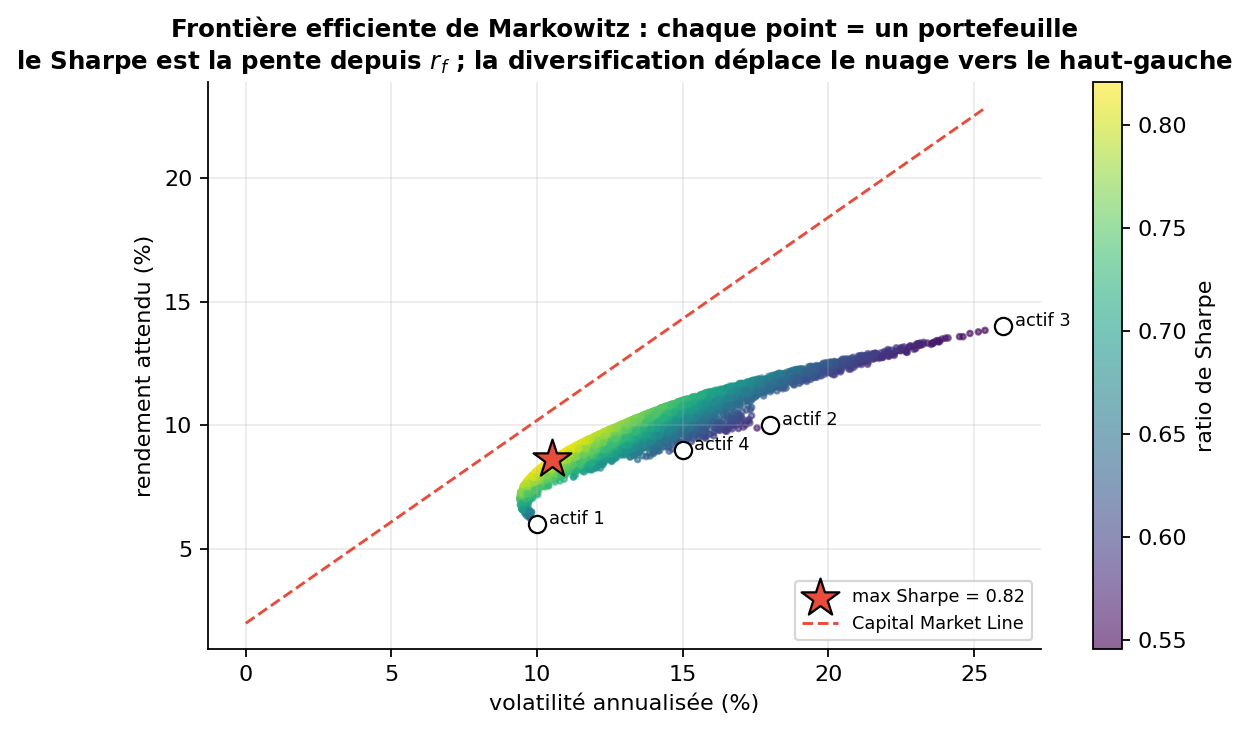
\includegraphics[width=0.82\textwidth]{fig_efficient_frontier.png}
\caption{Nuage de portefeuilles simulés sur quatre actifs. Le bord supérieur-gauche est
la frontière efficiente ; l'étoile est le portefeuille de \emph{Sharpe maximal}, point
de tangence de la \emph{Capital Market Line} issue de $r_f$. Le ratio de Sharpe est
géométriquement la \emph{pente} de la droite reliant $r_f$ à un portefeuille : le
maximiser, c'est trouver la droite la plus raide qui touche encore le nuage.}
\label{fig:frontier}
\end{figure}

Deux idées de ce cadre irriguent le projet. D'abord, le \textbf{ratio de Sharpe} que
j'utilise comme métrique n'est pas un choix arbitraire : c'est la pente de la CML,
l'unité naturelle du « rendement par unité de risque » dans ce modèle. Ensuite, la
\textbf{diversification} : parce que les actifs sont imparfaitement corrélés
($\Sigma$ n'est pas diagonale), un portefeuille a moins de risque que la moyenne de ses
composantes --- la seule « free lunch » de la finance. C'est exactement le mécanisme
que je retrouve, de façon inattendue, dans la robustesse au seed
(section~\ref{sec:seeds}) : moyenner l'alpha sur cinq actifs diversifie le bruit
d'entraînement idiosyncratique, comme un portefeuille diversifie le risque spécifique.
Mon environnement, lui, reste mono-actif (pas d'allocation) --- d'où un Sharpe
structurellement plafonné, et le projet « allocation sous contrainte CVaR » de ma liste.

\subsection{GARCH : modéliser le regroupement de volatilité}
\label{app:garch}

Les rendements financiers ne sont pas homoscédastiques : leur variance change dans le
temps et se regroupe (figure~\ref{fig:vol}). Le modèle GARCH(1,1) (Bollerslev, 1986,
généralisant l'ARCH d'Engle, 1982) capture ce fait par une variance conditionnelle
autorégressive :
\[
\sigma_t^2 = \omega + \alpha\,\varepsilon_{t-1}^2 + \beta\,\sigma_{t-1}^2,
\qquad \varepsilon_t = \sigma_t z_t,\quad z_t \sim \mathcal{N}(0,1) .
\]
La variance de demain est un mélange d'un socle $\omega$, du choc d'hier
$\varepsilon_{t-1}^2$ (terme ARCH) et de la variance d'hier $\sigma_{t-1}^2$ (terme
GARCH). La condition de stationnarité $\alpha + \beta < 1$ garantit un retour vers la
variance de long terme $\omega/(1 - \alpha - \beta)$ ; en pratique sur actions,
$\alpha + \beta$ est proche de 1 (volatilité très persistante). Je n'estime pas de
GARCH dans ce projet --- ma feature \code{volatility} en est un proxy non paramétrique
(l'écart-type glissant) --- mais c'est le modèle de référence auquel je comparerais une
prévision de volatilité (projet « GARCH vs ML » de ma liste), et le vocabulaire attendu
dès qu'on parle de risque conditionnel.

\subsection{Équation de Bellman : le socle de la fonction de valeur}
\label{app:bellman}

Pourquoi la fonction de valeur $V(s)$ (le critique de PPO) est-elle apprenable ? Parce
qu'elle satisfait une relation de cohérence récursive, l'\textbf{équation de Bellman} :
\[
V^\pi(s) = \mathbb{E}_{a \sim \pi,\, s'}\big[\, r(s, a) + \gamma\, V^\pi(s')\,\big] .
\]
« La valeur d'aujourd'hui = récompense immédiate + valeur actualisée de demain. » C'est
le principe d'optimalité de la programmation dynamique (Bellman, 1957) --- le même qui
sous-tend la résolution récursive d'un arbre de décision ou le pricing d'une option
américaine par backward induction. Le critique apprend $V$ en réduisant l'écart entre
ses deux membres (l'erreur de différence temporelle
$\delta_t = r_t + \gamma V(s_{t+1}) - V(s_t)$, brique de GAE en annexe~\ref{app:gae}).
Le pont avec la finance quantitative est direct : évaluer une option américaine, c'est
résoudre une équation de Bellman où « exercer » est une action et la valeur de
continuation joue le rôle de $\gamma V(s')$.

\end{document}
